\chapter{Analysis 3: Nonverbal Communication in Mining Debates}
\lhead{\textit{Analysis 3: Nonverbal Communication in Mining Debates}}

\textit{\textbf{Chapter Summary:} This chapter uses a multimodal corpus to consider nonverbal communication in the context of mining debates. This level of analysis gives insight into cognition and emotions in ways that textual data does not. These insights have important implications for the framing of environmental issues.}
\newline

\section{Multimodal, Nonverbal Communication}

The analyses in preceding chapters focus on language as text and, in the case of Analysis 2, textual representations of verbal communication. Of course, text is just one of many possible modes of human communication. While many insights can be gained from textual discourse analysis, the nuances and richness of human culture come to the fore when communication is multimodal. Multimodal communication draws from the textual as well as aural, linguistic, spatial, and visual capacities or modes \citep{Murray2013}. From a corpus linguistic and discourse analysis standpoint, multimodal implies consideration of a wider range of media such as audio, video, and images. It also implies the consideration and analysis of a broad spectrum of integrated human communication including nonverbal behaviors and paralanguage.  

This third and final analysis considers communication as an integrated whole. Speech and text segment language into constituent parts such that meaning is constructed from the bottom up, from words to phrases, and so on. By contrast, in the \textit{Lebenswelt} of everyday communication, it is the combination of fluid verbal and nonverbal semiosis that creates meaning. Estimates of the degree to which human communication is nonverbal have varied. Depending on the context, it has been suggested that over 90 percent of communication is nonverbal \citep{Mehrabian1972}, but this figure depends highly on the context and is not a universal claim. Elsewhere, it has been suggested two-thirds of all communication is nonverbal \citep{Burgoon2016}. Regardless, of the exact estimates, it suffices to say that nonverbal communication is integral to overall meaning and understanding.

Nonverbal can refer to a wide range of information transfer through visual, auditory, tactile, and kinesthetic channels. For this present analysis, however, we focus particularly on gestures and facial expressions. Paralanguage, such as pitch and intonation, will also be considered secondarily. In addition, nonverbal communication is considered alongside speech rather than in isolation. The rationale for not isolating the nonverbal is that verbal statements provide necessary context to interpret the meaning of gestures and expressions. Each of the elements (gesture, facial expression, paralanguage, etc.) is a vast, specialized topic. The present aim, therefore, is a more general interpretation of holistic communicative acts.

\section{Corpus Data}

From a corpus linguistics and discourse analysis standpoint, multimodal implies the consideration and analysis of a broad spectrum of integrated human communication including nonverbal behaviors. More precisely, a multimodal corpus is defined by \cite*{Foster2008} as

\begin{quote}
an annotated collection of coordinated content on communication channels such as speech,
gaze, hand gesture, and body language, [that] is generally based on recorded
human behaviour (4).
\end{quote}

Thus, in addition to the data itself (i.e. recorded human behaviour), annotation of the multimodal corpus is a defining feature. However, annotation is a challenge for multimodal corpus research given both the time it requires as well as the lack of annotation standards \citep{Abuczki2013}.

For Corpus 3, the recorded human behaviour consists of audio and video representing different perspectives on mining and natural resource development. These include interviews, documentaries, recordings of `town hall' type meetings. The data was collected manually using a search engine (most results were from \textit{YouTube} and some from archives of news broadcasting agencies). Transcripts were then obtained for each media item and saved as separate files (\textit{txt} format).

There are 25 files in total, each with a url associated back to the original audio/visual media. The transcripts include timestamps (e.g. 05:45). By looping through the transcripts and getting the last timestamp, the total runtime of the media was calculated as 7 hours 46 minutes. The average runtime is about 18 minutes.

Rather than annotating the entire corpus, selections were obtained using both top-down and bottom-up approaches. In the top-down approach, the media was watched/listened to manually, paying close attention to gesture, body language, or other non-verbal expressions. Timestamps of interest (i.e. points in the recording with distinctive and pronounced non-verbal expression) were then marked for further annotation. The bottom-up approach began by searching for keywords and phrases related to analytical themes (i.e. ecology, culture, socio-economic). Segments related to key themes were then identified for further analysis and annotation. 

The next step was interpretation and analysis. There are competing theories concerning the meaning and interpretation of nonverbal communication (NVC). Topics of debate include the extent to which nonverbal behaviours are universal by virtue of our common biological or evolutionary origins, or the degree to which they are culturally variable \citep[e.g.][]{Jack2012}. Also debated is whether nonverbal behaviors are reflective of internal, cognitive states or whether they are better understood in terms of social interaction and influence \citep[e.g.][]{Crivelli2018}. These debates are touched upon in this chapter, but their details are generally beyond the current scope.

The present analysis aims, first and foremost, to be descriptive. Nonverbal analyses of this specific genre (i.e. environmental communication) are limited. Comparative data and observations are, therefore, valuable, even if interpretation is limited. The descriptive segments consist of video transcripts with annotations, together with footnote physical descriptions of nonverbals. The annotation method used is based on that of \cite{Jefferson2004}, as summarized in Table 5.1. Image frames from the video segments are also included.

Following each description is a brief interpretive narrative. The purpose of the narrative is to tie together the various NVC elements as well as integrate them with the verbal component. These narratives generally include some discussion, based on secondary literature, of what the nonverbals \textit{could} mean. Considering gestures, facial expressions, paralanguage, together with the verbal language, the following questions guide interpretation:

\begin{itemize}
\item What does the NVC tell us about the emotional state of the speaker?
\item How does the NVC complement, or contrast with, the verbal communication?
\item Does NVC give insight into how the speaker is thinking?
\end{itemize}

Following the descriptions and interpretations of each segment, comparison and analysis across all the segments is conducted.   

\begin{table}[H]
\begin{footnotesize}
\centering
\def\arraystretch{1.1}% 
\begin{tabular}{ | P{2cm} P{3cm} P{6cm}|}  
\hline
(.)             & Micro-pause                    & A brief pause, usually less than 0.2 seconds.                                                                      \\ \hline
. or down arrow & Period or Down Arrow           & Indicates falling pitch or intonation.                                                                             \\ \hline
? or up arrow   & Question Mark or Up Arrow      & Indicates rising pitch or intonation.                                                                              \\ \hline
,               & Comma                          & Indicates a temporary rise or fall in intonation.                                                                  \\ \hline
!-              & Hyphen                         & Indicates an abrupt halt or interruption in utterance.                                                             \\ \hline
>text<          & Greater than/Less than symbols & Indicates that the enclosed speech was delivered more rapidly than usual for the speaker.                          \\ \hline
<text>          & Less than/Greater than symbols & Indicates that the enclosed speech was delivered more slowly than usual for the speaker.                          \\ \hline
\degree         & Degree symbol                  & Indicates whisper, reduced volume or quiet speech.                                                                 \\ \hline
ALL CAPS        & Capitalized text               & Indicates shouted or increased-volume speech                                                                       \\ \hline
underline       & Underlined text                & Indicates the speaker is emphasising or stressing the speech.                                                      \\ \hline
:::             & Colon(s)                       & Indicates prolongation of a sound.                                                                                 \\ \hline
hhh             &                                & Audible exhalation                                                                                                 \\ \hline
.hhh            &                                & Audible inhalation                                                                                                 \\ \hline
(text)          & Parentheses                    & Speech which is unclear or in doubt in the transcript.                                                             \\ \hline
[text]          & Square brackets                & Speech within square brackets is accompanied by the meaningful part of the gesture - the so-called `stroke phase'. \\ \hline
\end{tabular}
\caption{Gail Jefferson's (\citeyear{Jefferson2004}) annotation scheme as adapted by \cite[5]{Beattie2016}}
\label{tab:table1}
\end{footnotesize}
\end{table}

\section{Multilevel Analysis}

Compared to the corpora covered in the previous two chapters, there are a number of considerations in light of a multimodal corpus. The first difference concerns the blending of topics. In previous chapters, the levels of analysis are segmented (ecological, cultural, socio-economic, cognitive). Textual corpora allow for this segmentation as the topics of discourse could be discerned at the sentence level. This separation continues in this chapter, but the multimodal corpus highlights the extent to which the levels blend in the normal flow of verbal communication. In the text corpora, there are often definitive boundaries between themes. By contrast, in this corpus it is common to find a combination of cultural, socio-economic, and ecological themes within a single phrase. This makes segmentation of levels more difficult than it was in Analyses 1 and 2. 

There are also differences in the language itself. Since data from the multimodal corpus consist entirely of spoken/conversational language, differences from the other (textual) corpora can be expected. While the extent to which there are sharp differences between written and spoken English is debatable \citep{Biber1988}, one might expect a spoken language corpus to include shorter, simpler sentences, less lexical diversity, less nomialization (usage of nouns versus verbs), and high contextualization.   

A keyword analysis of the corpus transcripts points to some of these language differences. Recall that in both Analyses 1 and 2, keywords were indicative of overall themes and often contained rich, specialized lexical items. In the present corpus, the top ten keywords are: \textit{know}, \textit{people}, \textit{right}, \textit{mining}, \textit{think}, \textit{one}, \textit{like}, \textit{mine}, \textit{say}, \textit{going}, and \textit{year}. With the possible exception of \textit{mining} and \textit{mine} these keywords are very generic and hardly indicate overall discourse themes. These results are indicative of the highly contextual nature of spoken language. The contextual nature of the multimodal data means that, in analysis and interpretation, less emphasis can be placed on lexical items. Consider that the previous two analyses began by looking at lexical items. Keywords and concordance lines were used to isolate points of interest in the data. These points of interest were then examined in more detail to infer patterns of meaning in the communication. While, this present analysis will also draw on lexical items (from transcripts), it does not rely on text to the same degree. 

Rather than lexical items, points of interest are identified from segments which contain particularly expressive nonverbal communication. The aim of selecting segments from the multimodal data is to identity moments where speech and nonverbal expressions combine to underscore meaning. These moments are what \cite*{McNeill2005b} calls points of ``highest communicative dynamism'' (1). 

In the present analysis, we examine multimodal communication through source data consisting of about 8 hours of video segments. From the 8 hours of video, 13 clips were selected for annotation and detailed analysis. Although the segments are diverse in length and genre, they share a common theme; namely, mining development. The segments include interviews, round table discussions, town hall meetings, etc. on the topics of deep sea mining, uranium mining, mountain top coal mining, mineral extraction and economic development, and other related themes. 

The analysis that follows presents 4-6 examples for three of the levels: ecological, cultural, and socio-economic. Rather than presenting separate examples from the cognitive-level, the cognitive analysis will go deeper into the segments presented in the first three levels.

\subsection{Ecological Level}

For the ecological level, excerpts were selected wherein speakers are explicitly discussing ecological issues. These excerpts are not based on keywords and concordances (as in the previous analyses), but were selected manually, from a qualitative survey of the data. Despite the nearly 8 hours of video on the topic of natural resource development, there are relatively few cases where the speech segments clearly fell into the ecological level, meaning there are not coinciding political, cultural, economic themes within the excerpts.

Below there are four examples of ecological-level communication. Three of these excerpts feature subject matter experts who employ technical and scientific concepts. The final example features a citizen protester. Example 1 below consists of an excerpt and accompanying gestures in Figure 5.1. In this segment, a researcher is discussing impacts of deep sea mining.

\textbf{\underline{Ecological Level - Example 1}}

\begin{footnotesize}

\texttt{(the) [\annotate{direct} impact]\textsuperscript{1} will likely result in biodiversity loss that will be very difficult to [recover from,]\textsuperscript{2} but we \annotate{really} don't understand is any of the [\annotate{wider} impacts]\textsuperscript{3} as well, so outside the [area of]\textsuperscript{4} mining itself <how will this> [affect the ecosystem at large how will this feedback into the oceans]\textsuperscript{5} we think that the deep sea...}

\end{footnotesize}

\begin{footnotesize}
\begin{enumerate}
   \item Hand downward in swift movement, fingers pointed outward
   \item Hands in cycling motion forward
   \item Hands expanding outwards
   \item Hand in wide circular movement with palm down
   \item Hands in cycling movement with palms inwards
\end{enumerate}
\end{footnotesize}

\begin{figure}[H]
\centering
\begin{tabular}{llll}
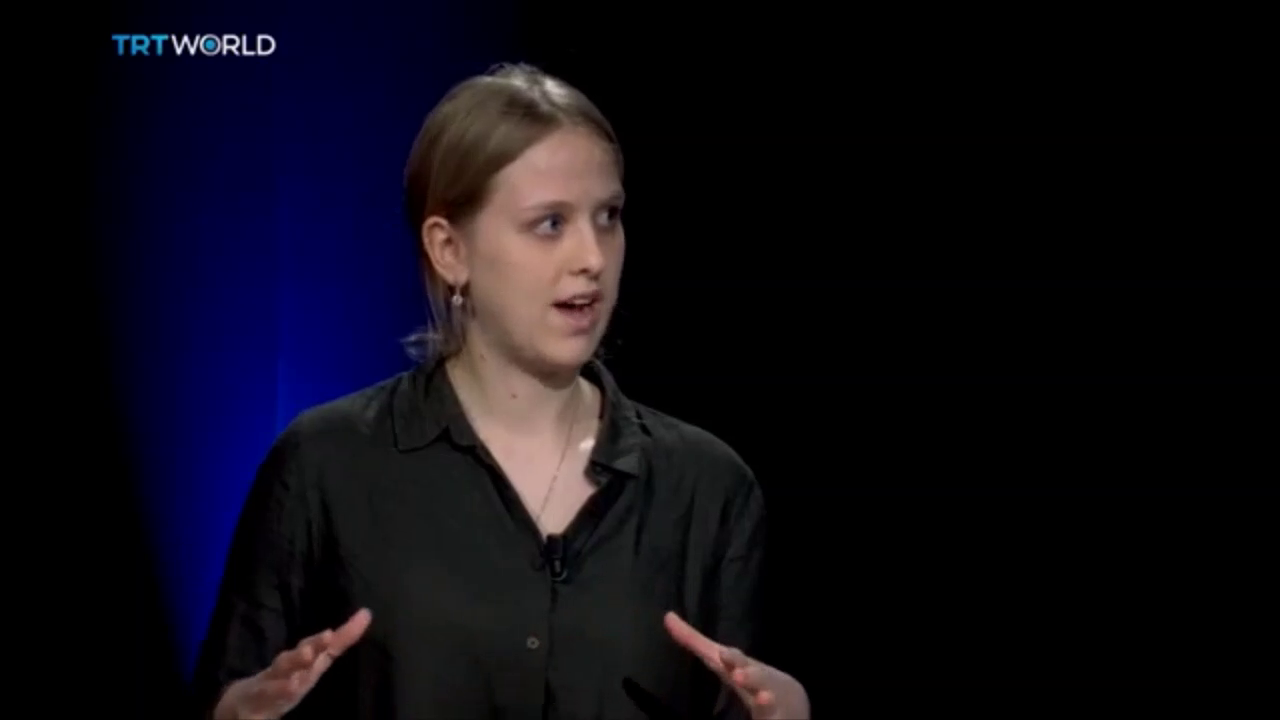
\includegraphics[width=4.2cm]{Figures/mmEco/frame207.png} & 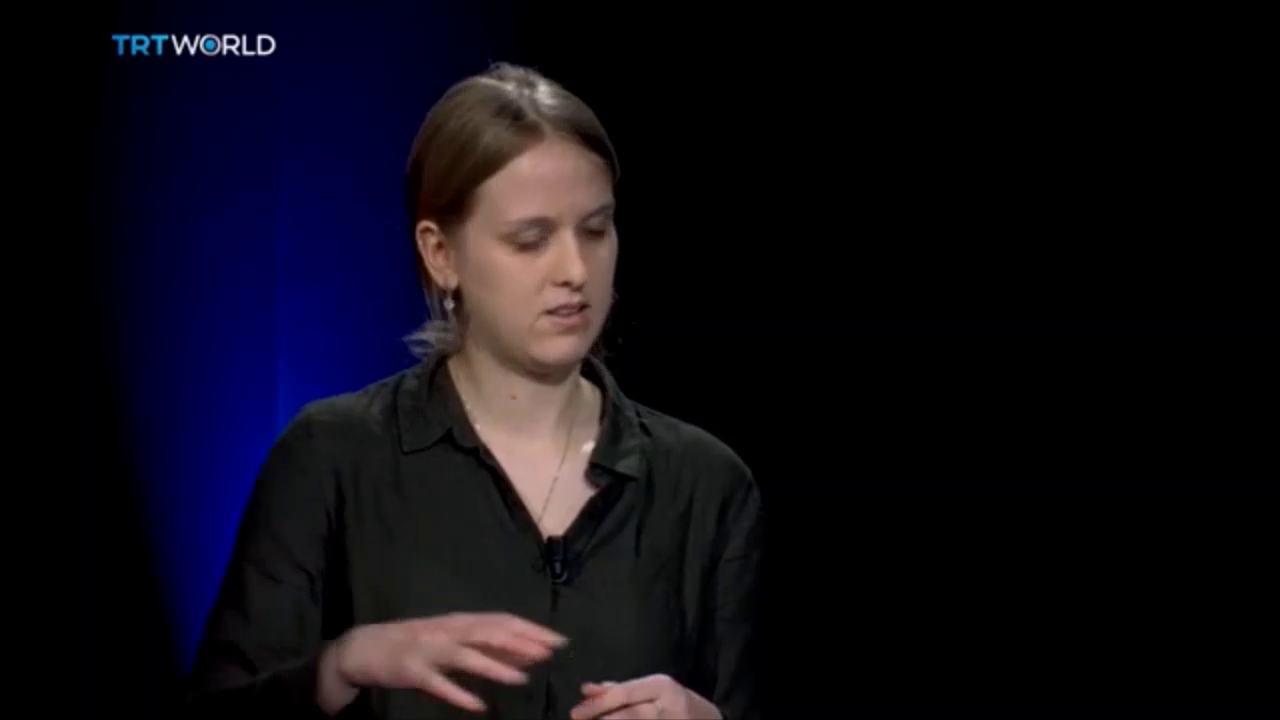
\includegraphics[width=4.2cm]{Figures/mmEco/frame252.png} & 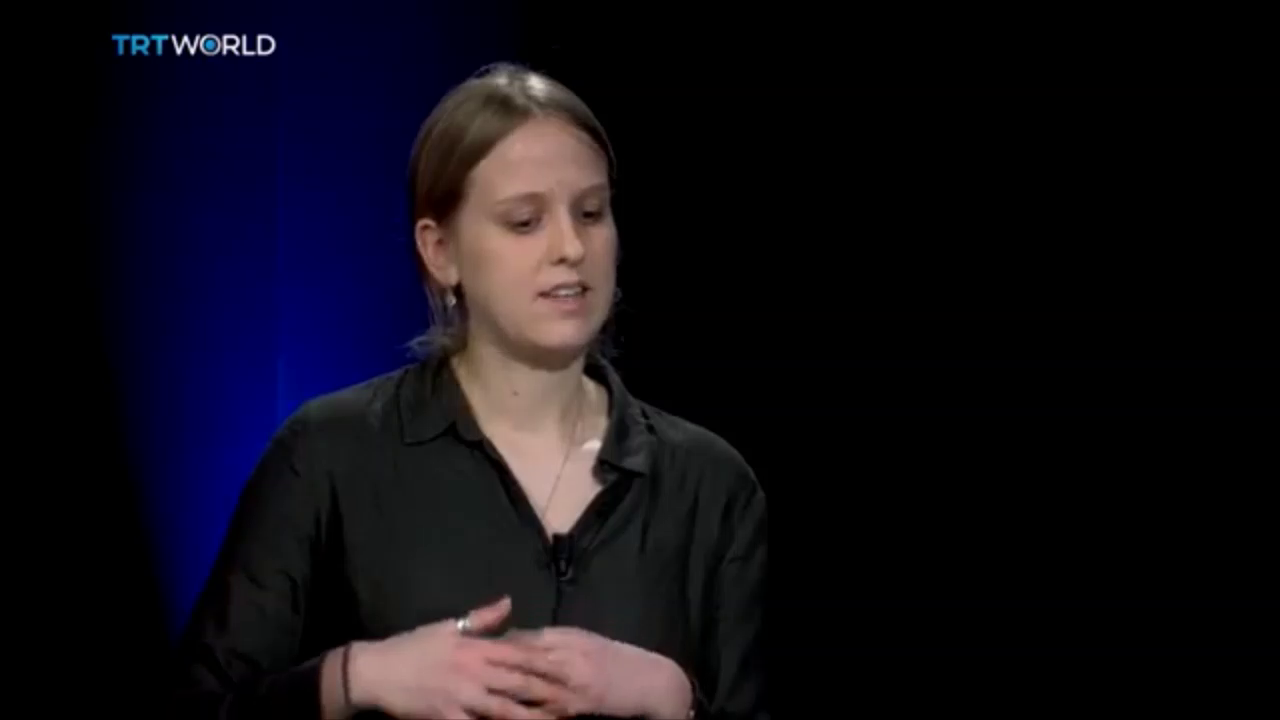
\includegraphics[width=4.2cm]{Figures/mmEco/frame392.png} 

\end{tabular}
\caption{Ecological Level - Example 1}
\begin{footnotesize}
Left: hands open palms down gesture with fingers extended to emphasize direct ecological impacts. Middle, Right: Hands loosened, palms inward/down in a cycling motion to reflect less certain long term ecological processes and feedback mechanisms.\\

Source: \url{https://www.youtube.com/embed/-UPjsuuyvD4?start=632&end=653}
\end{footnotesize}
\label{fig:figure1}

\end{figure}

Noticeable in Example 1 are the controlled hand gestures. The hands reflect the physical and ecological processes taking place. For instance, ``direct impact'' of mining is accompanied by a swift downward movement or arms and hands. The fingers and thumbs extended with palms facing downward are indicative of impact and gravity in a short time frame. When speaking of the ``area of mining'' the palm is similarly facing downward with a circular motion of the hand, indicating surety of the impacts in the mining area. By contrast, the cycling motions of the hands indicate a longer time frame of ``feedback'' and wider impacts. The palms shift to face inwards with more relaxed (non extended) fingers and thumbs, suggesting less certainty about these long term impacts. So, in this excerpt we see how the direction of palms and extension of fingers/thumbs reflect degrees of certainty and uncertainty.

Beyond hand gestures, other nonverbals are noticeable. For much of the segment the head is tilted to the side, which has been interpreted as a sign of interest, curiosity, and uncertainty \citep[94]{Lewis2012}. There are moments where the eye gaze shifts upwards which, in  European/North American cultures is commonly seen as a sign that someone is thinking \citep{McCarthy2006}. Finally, it should be noted that facial expressions in Example 1 are minimal and do not convey any apparent emotions. 

Example 2 features a researcher talking about concerns associated with coal mining near a nature reserve. 

\textbf{\underline{Ecological Level - Example 2}}

\begin{footnotesize}
\texttt{Where our [concern lies is with respect to \annotate{dust}!- because there's no analysis of the dust(.) in terms of the toxic components in that dust]\textsuperscript{1} given the coal mining and the blasting and that sort of thing\degree. Now, you can feel [\annotate{this wind}. <This wind>]\textsuperscript{2} (.) is blowing across us [right into the game reserve]\textsuperscript{3}, so [if] they mine here, this south-easterly wind will carry the dust and the fallout will be in the park, >in the wilderness area<.}   
\end{footnotesize}

\begin{footnotesize}
\begin{enumerate}
   \item Hand in front facing inwards palms open thumbs up
   \item Hands pointing left hand to left
   \item Hand (right) pointing to the right
\end{enumerate}
\end{footnotesize}

\begin{figure}[H]
\centering
\begin{tabular}{llll}

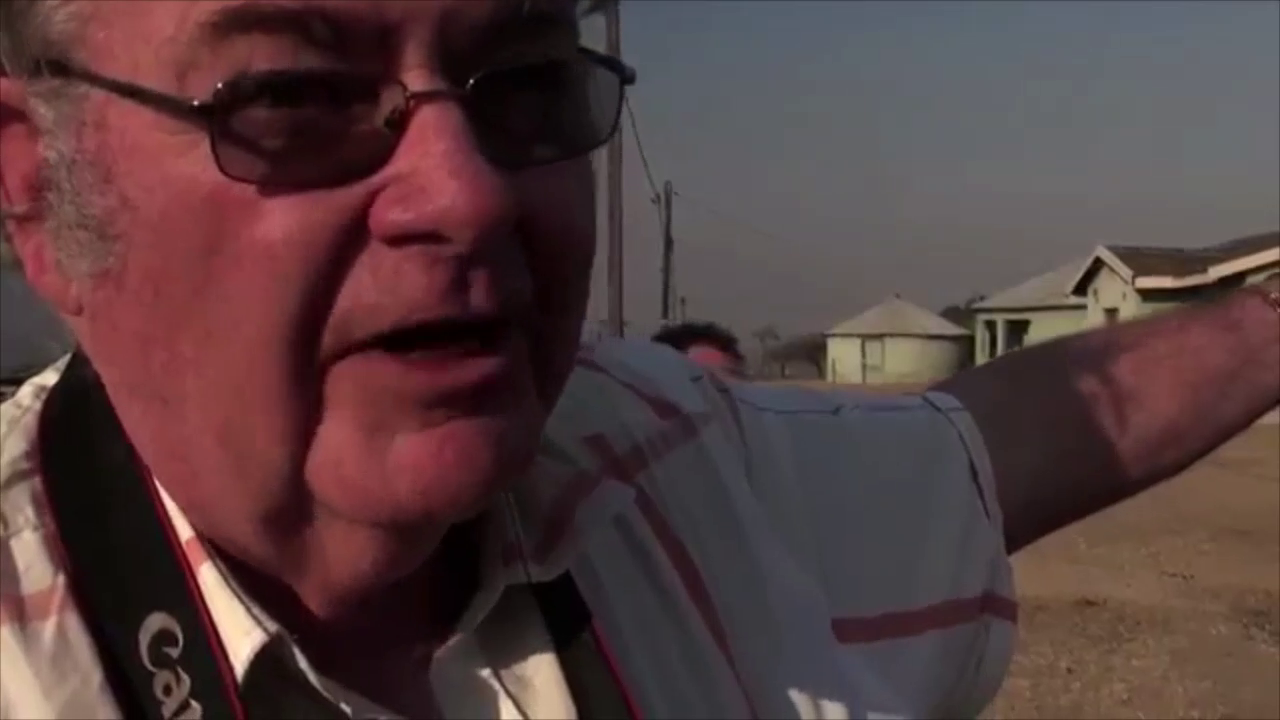
\includegraphics[width=4.2cm]{Figures/mmEco1/frame578.png} & 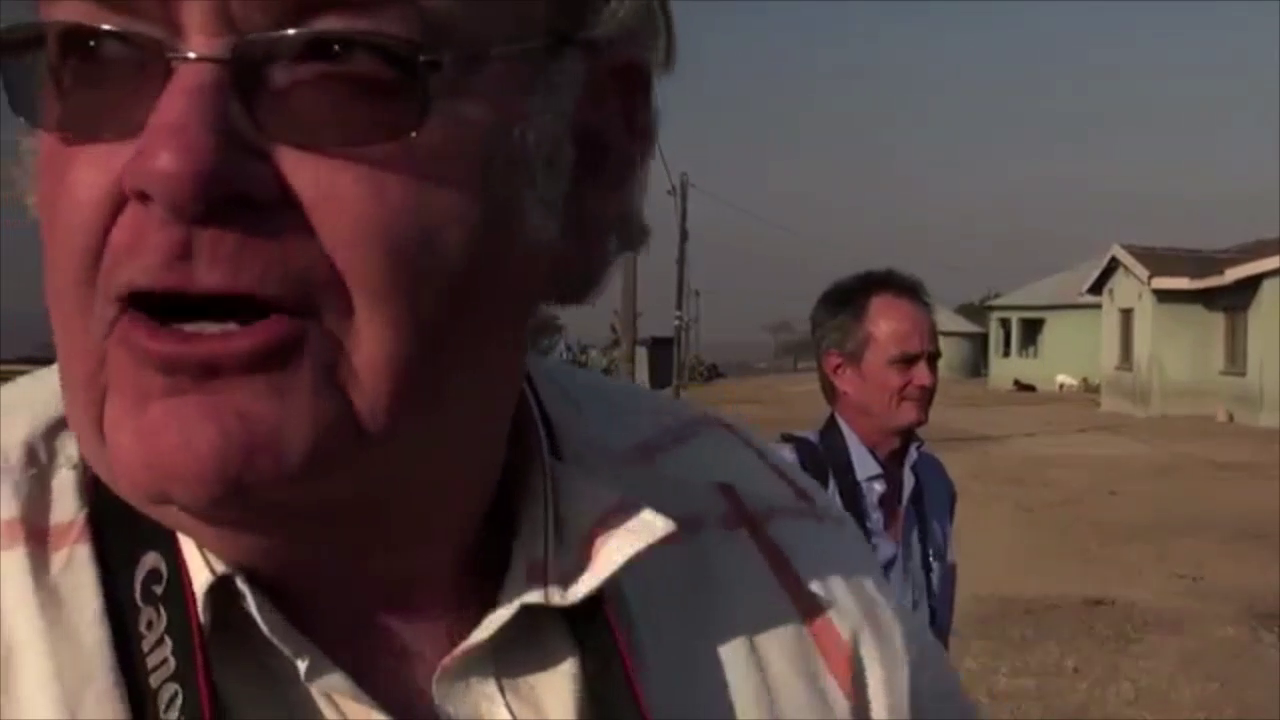
\includegraphics[width=4.2cm]{Figures/mmEco1/frame619.png} & 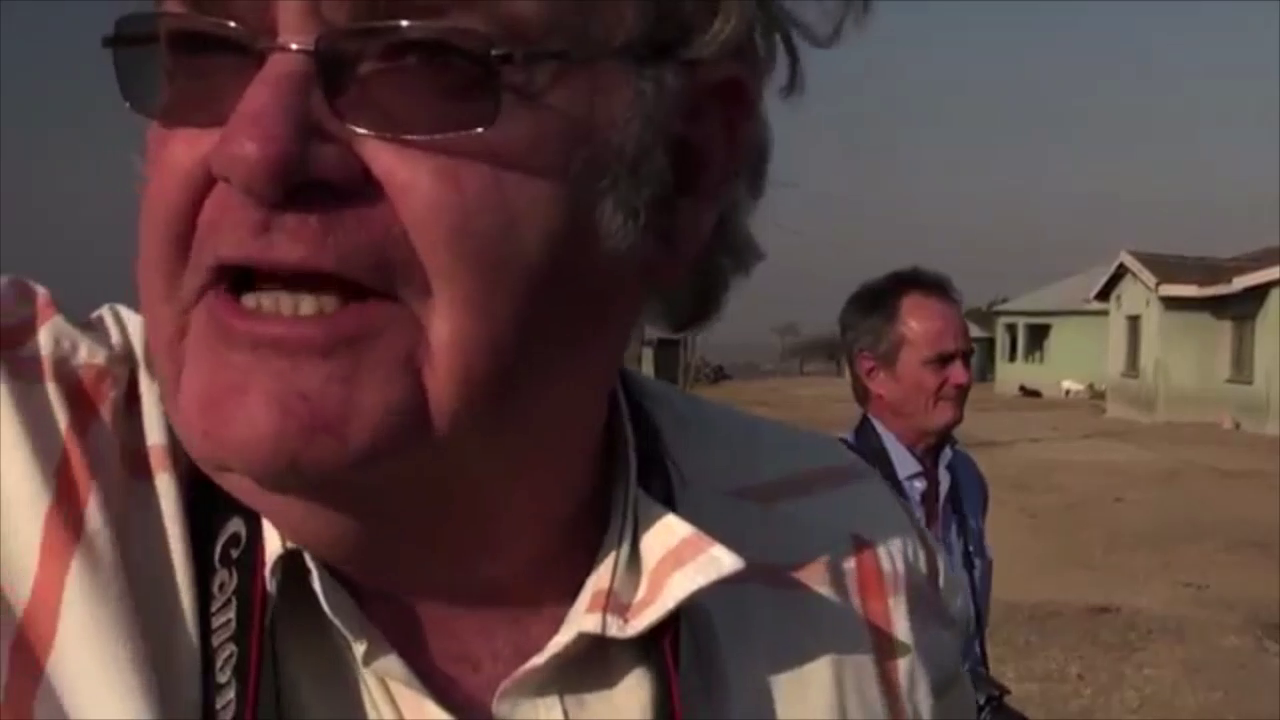
\includegraphics[width=4.2cm]{Figures/mmEco1/frame634.png}  

\end{tabular}
\caption{Ecological Level - Example 2}
\begin{footnotesize}
Hand and arm points to left (Left image) and then to right (Right image) to reflect the physical movement of dust.\\

Source: \url{https://www.youtube.com/embed/Sh0_Wf8F4RM?start=857&end=888)}
\end{footnotesize}
\label{fig:figure1}
\end{figure}

Though difficult to see in the frame, when the man in Example 2 is speaking about ``our concern,'' the palms are inward. The fingers and thumbs are extended and the hands motioning up and down with speech emphasis. This cluster of hand gestures suggests possession (palms inward to express \textit{our} concern)  as well as a confidence that this is serious (thumbs up) perhaps with a degree of uncertainty (palms inward). Also, as in the previous excerpt, the hands and arms are used to describe physical and ecological processes which, in this case, is the directional transfer of dust.  

Compared with Example 1, there are several indicators in Example 2 suggesting the speaker's emotions are at play. In the first excerpt, hand movements are used to complement and reiterate the verbal communication. On the second, however, the nonverbals give more of an indication about what is not explicit verbally. For instance, the furrowed eyebrows indicate stress and concern, as do stress lines on the forehead. The swift, agitated up and down movement of hands also convey a sense of urgency. The speaker places stress on certain words (e.g. ``dust'', ``wind'') and changes the speed and cadence.    

In Example 3, an engineer or industry representative is facing questioning on contamination of groundwater due to coal mining. 

\textbf{\underline{Ecological Level - Example 3}}

\begin{footnotesize}
\texttt{People don't understand that <you have to> >[maintain a well just like you do your \annotate{car}]<.\textsuperscript{1} A lot of people just [turn on the spigot,]\textsuperscript{2} and they think [it's going to work for them]\textsuperscript{3} (.) when they have <things like iron hydroxide precipitate> (.) and other metals built up in [their wells (and) every time I go out on a well complaint, I tell people]\textsuperscript{4} you [need to have a friend at the local (.) volunteer fire department come out and flush your well (out)]\textsuperscript{5}....}  
\end{footnotesize}

\begin{footnotesize}
\begin{enumerate}
   \item Index finger and thumb together in precision
   \item Turning of index finger and thumb 
   \item Hand out palm up 
   \item Hand out palm up 
   \item Nodding
\end{enumerate}
\end{footnotesize}

\begin{figure}[H]
\centering
\begin{tabular}{llll}


\includegraphics[width=4.2cm]{Figures/mmEco2/frame182.png} & 
\includegraphics[width=4.2cm]{Figures/mmEco2/frame207.png} & 
\includegraphics[width=4.2cm]{Figures/mmEco2/frame286.png}  

\end{tabular}
\caption{Ecological Level - Example 3}
\begin{footnotesize}
Left and Middle: the index finger and thumb join to create a precision movement. Right: the open hand palm up gesture functions as a suppliant offer of an idea.\\
Source: \url{https://www.youtube.com/embed/UvKe2LYy5pk?start=920&end=945}
\end{footnotesize}
\label{fig:figure1}
\end{figure}

In the context of the segment, the speaker is on the defensive, since he is trying to convince listeners that the coal industry is not responsible for water quality issues. A noticeable gesture is the touching of the thumb and index finger, which is accompanied by a turning motion when describing well operation. Like in the previous examples, hand gestures complement and emphasize the verbal communication by mimicking physical processes. Touching the index finger and thumb is also used in Western cultures to emphasize a point. The ring shape has been described by \cite{Kendon2004} and others as indicating precision. A possible effect of this gesture here is to focus and narrow the discussion to one of specific technical expertise.

In later frames, the speaker extends the right hand out with fingers extended and the palm rotated upward. The palm up is used for a variety of nuanced meanings including uncertainty, emphasis, emotional helplessness, and social deference \citep{GivensDavidB2016}. \cite{Muller2004} suggests that the function of the open hand palm up gesture is to present an idea for consideration. Here, the gesture functions as a non-forceful convincing plea. Given the context, one could interpret the palm up gesture as a rhetorical device, intended to convince and influence listeners. Other nonverbals might be interpreted in this way, as rhetorical, including the slight smile in early frames as well as a nodding at the end of the segment. The smile, it has been argued, is a way to appear nonthreatening to others \citep{Cunningham2004}. Nodding can be seen as a way to build rapport and activate mirroring between the speaker and listeners.

Example 4 is unique because of the constrained position of the speaker. This segment was filmed after protesters had been arrested and placed in hand restraints (Figure 5.4, Left). 

\textbf{\underline{Ecological Level - Example 4}}

\begin{footnotesize}
\texttt{[We've got to build a whole new energy infrastructure for this country, and if we don't we're going to have (.) climate chaos and our kids are going to \annotate{not} thank us for that].\textsuperscript{1}}
\end{footnotesize}

\begin{footnotesize}
\begin{enumerate}
   \item Continuous shaking of HEAD
\end{enumerate}
\end{footnotesize}

\begin{figure}[H]
\centering
\begin{tabular}{llll}

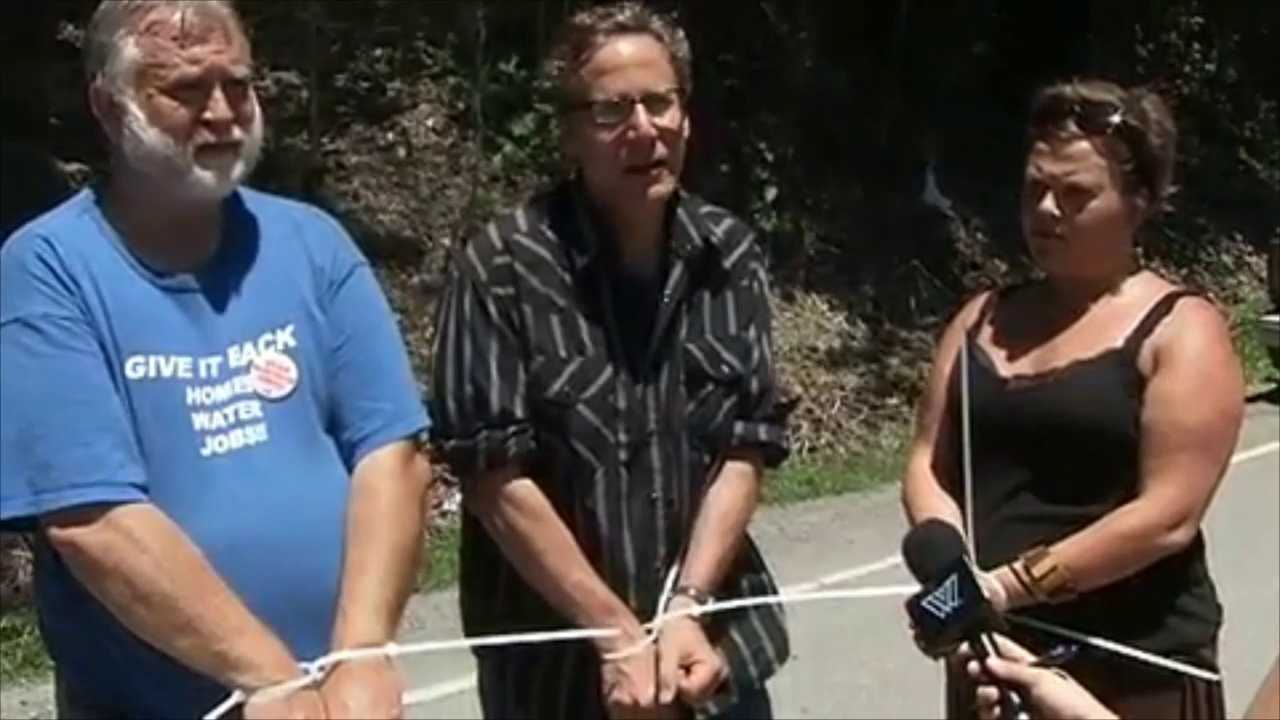
\includegraphics[width=4.2cm]{Figures/mmEco4/frame8.png} & 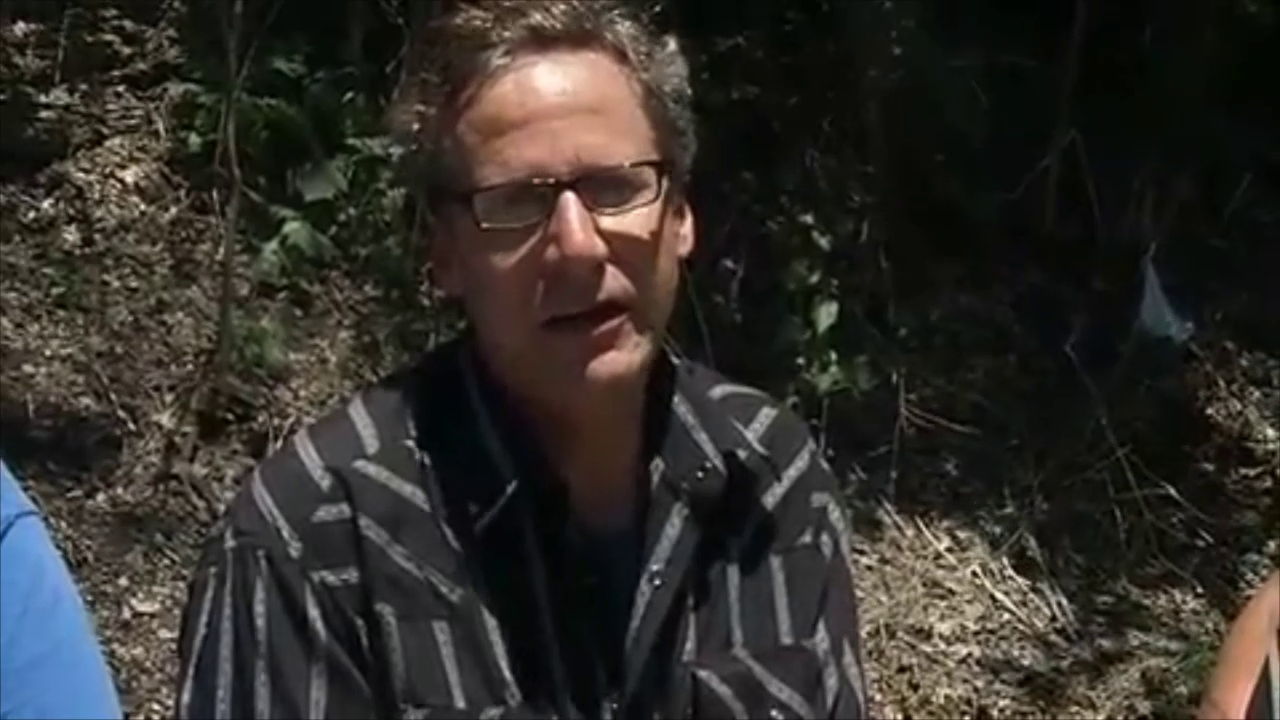
\includegraphics[width=4.2cm]{Figures/mmEco4/frame192.png} & 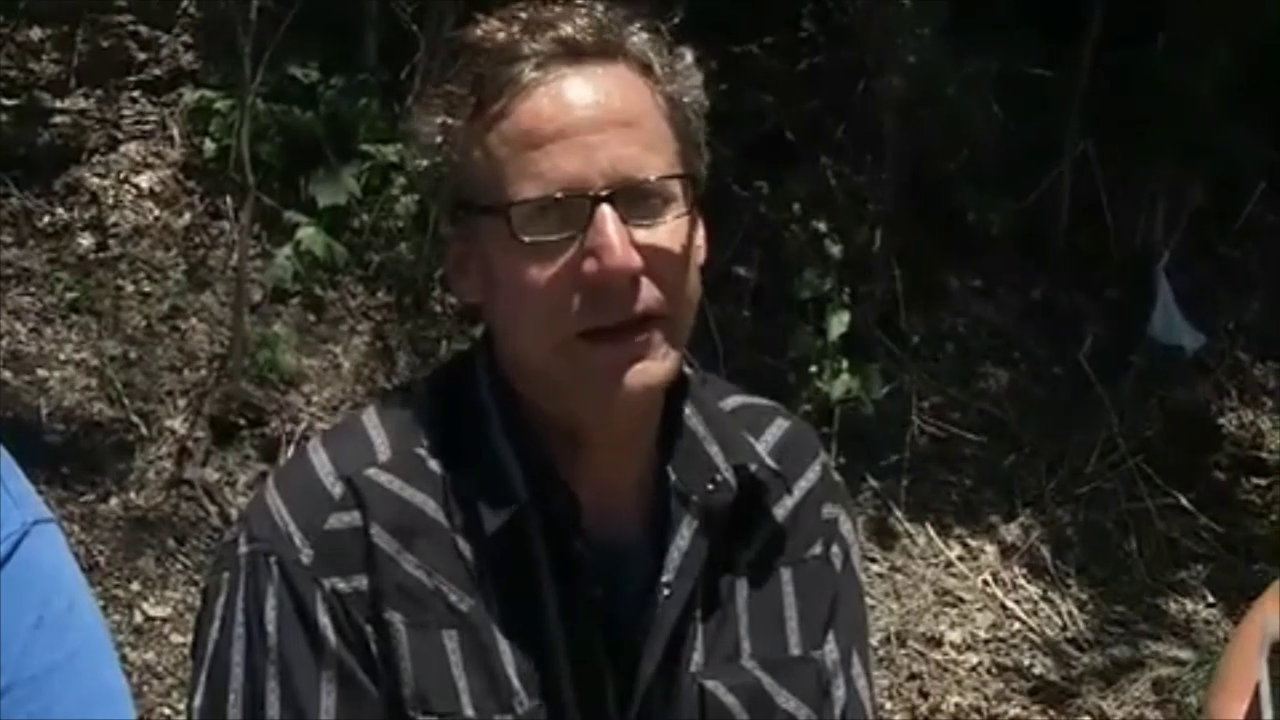
\includegraphics[width=4.2cm]{Figures/mmEco4/frame219.png}  

\end{tabular}
\caption{Ecological Level - Example 4}
\begin{footnotesize}
Left: hands constrained, possible accentuating communicative head movements. Middle, Right: continuous movement (shaking) of head from left to right carrying the meaning of unbelievable.\\
Source: \url{https://www.youtube.com/embed/vBhvFWRLiOs?start=821&end=829}
\end{footnotesize}
\label{fig:figure1}
\end{figure}

With the hands immobilized, gestures in Example 4 are confined largely to the head. In this segment, the speaker is expressing the need to build new energy infrastructure in the face of climate change. The words are accompanied by continuous shaking of the head. This head gesture might be interpreted as disapproval and condemnation. However, it can also be considered that this head shaking functions as a verbal intensifier with the negation carrying the meaning of ``unbelievable'' \citep[861]{McClave2000}. Also noticeable in this clip is the slight head tilt (also seen in Example 1). The facial expression might be interpreted as serious and sombre, but does not display a high degree of emotion.

\textbf{Summary of Ecological-Level}

The four examples above feature speakers from different points of view with respect to the ecological issues at hand. Of the four speakers, two are researchers, one is a company representative, and another is a protester. In all cases, the level of emotion expressed through nonverbal communication is minimal. While the second speaker does appear to convey some agitation or urgency through facial expressions and paralanguage, the overall segment is more a rational argumentation than an emotional expression. The last speaker, despite the context of being arrested, comes across as sombre and earnest, but not particularly emotional.

In the first three examples, gestures are predominantly iconic speech illustrators, meaning they display a close relationship with the content of the speech \cite[60]{Beattie2016}; \cite[76]{Matsumoto2012}. For instance, the first speaker uses deliberate and measured hand movements that reflect biophysical processes (ecological impact, recovery) expressed in speech. Also in Example 2, hand gestures reflect physical processes of dust transfer. The third speaker uses nonverbal hand movements to reflect the process of inspecting a well, but also employs what could be described as rhetorical gestures to convince listeners. 

\subsection{Cultural Level}

Examples in the cultural-level feature people expressing their cultural identities in some way. These identities take on different forms including national, sub-national/regional, ethnic, and religious. In Example 1, national cultural identity is being discussed in the context of resource development and cultural preservation in Afghanistan. Examples 2 and 3, invoke indigenous ancestry. In the case of Example 4, religion and spirituality come into play. Finally, in Example 5 we see an expression of local/regional identity.

The first example below is from a report on cultural heritage and extractive mining in Afghanistan. The segment is an interview with an Archaeologist who, based on his use of the phrase ``our identity,'' clearly identifies with Afghan culture.

\textbf{\underline{Cultural Level - Example 1}}

\begin{footnotesize}
\texttt{...with [all these wars (over) 30, 40 years]\textsuperscript{1}, (.) what the Afghan has lost we lost [our identity]\textsuperscript{2}!- and [I \annotate{believe}]\textsuperscript{3} to give (them) \annotate{back} that identity is only through [\annotate{culture}]\textsuperscript{4} !- because when it [\annotate{comes}]\textsuperscript{5} to culture, all Afghans are united.}
\end{footnotesize}

\begin{footnotesize}
\begin{enumerate}
   \item Left hand forward palm up; lateral sweep of head and hand
   \item Right hand motion to side; index finger extended; eyebrows raise
   \item Right hand motion to side; index finger extended; head tilts to one side
   \item Right hand motion forward; index finger extended
   \item Right hand motion forward; index finger extended; intonation on ``comes''
\end{enumerate}
\end{footnotesize}

\begin{figure}[H]
\centering
\begin{tabular}{llll}
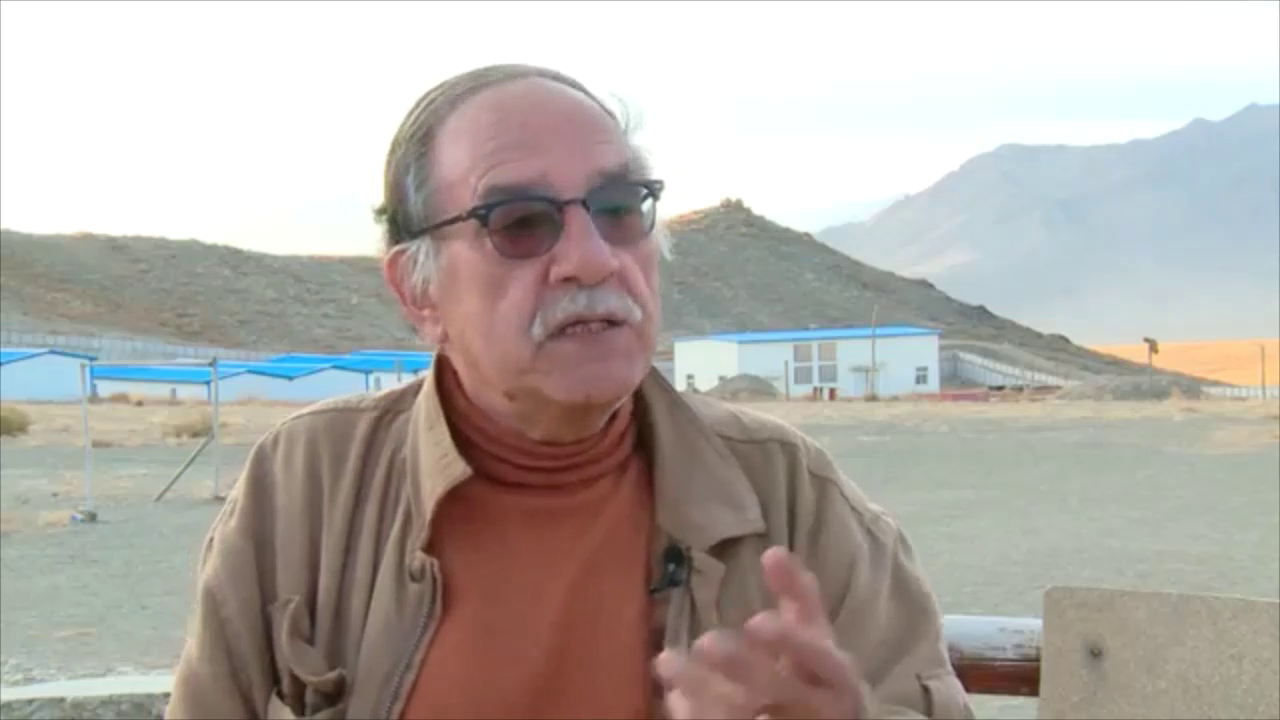
\includegraphics[width=4.2cm]{Figures/mmCult1/frame15.png} & 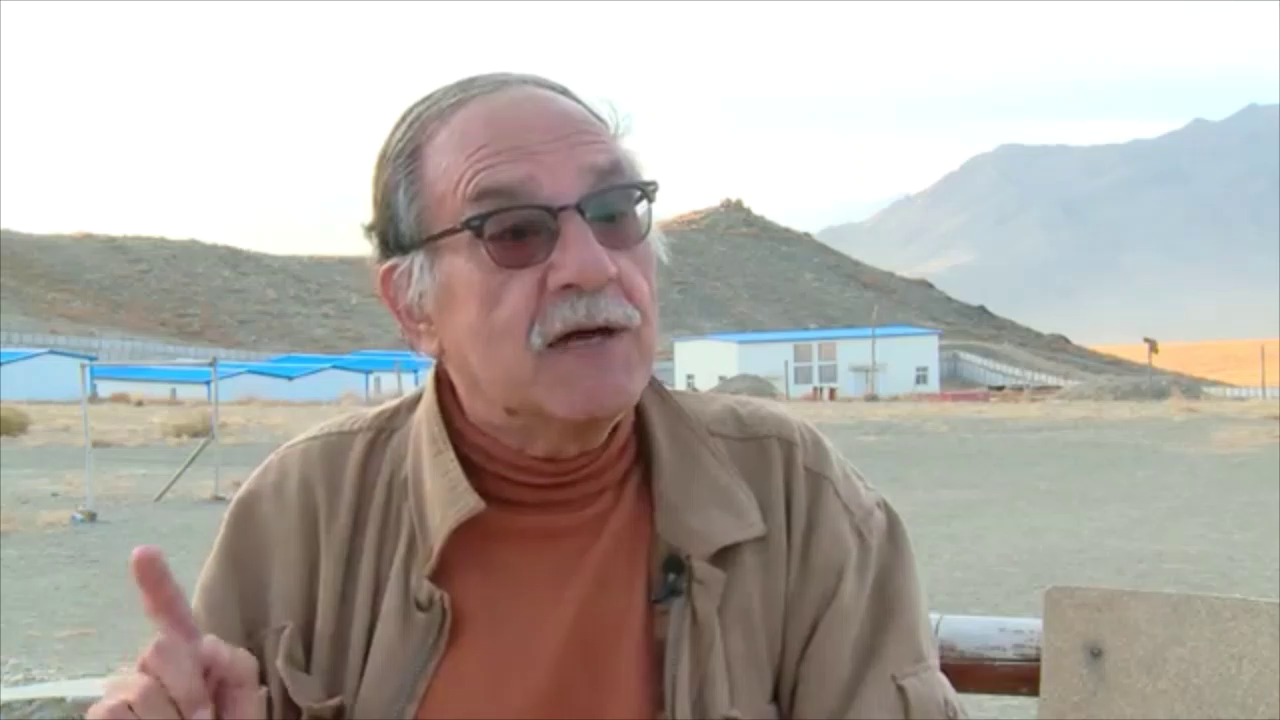
\includegraphics[width=4.2cm]{Figures/mmCult1/frame241.png} & 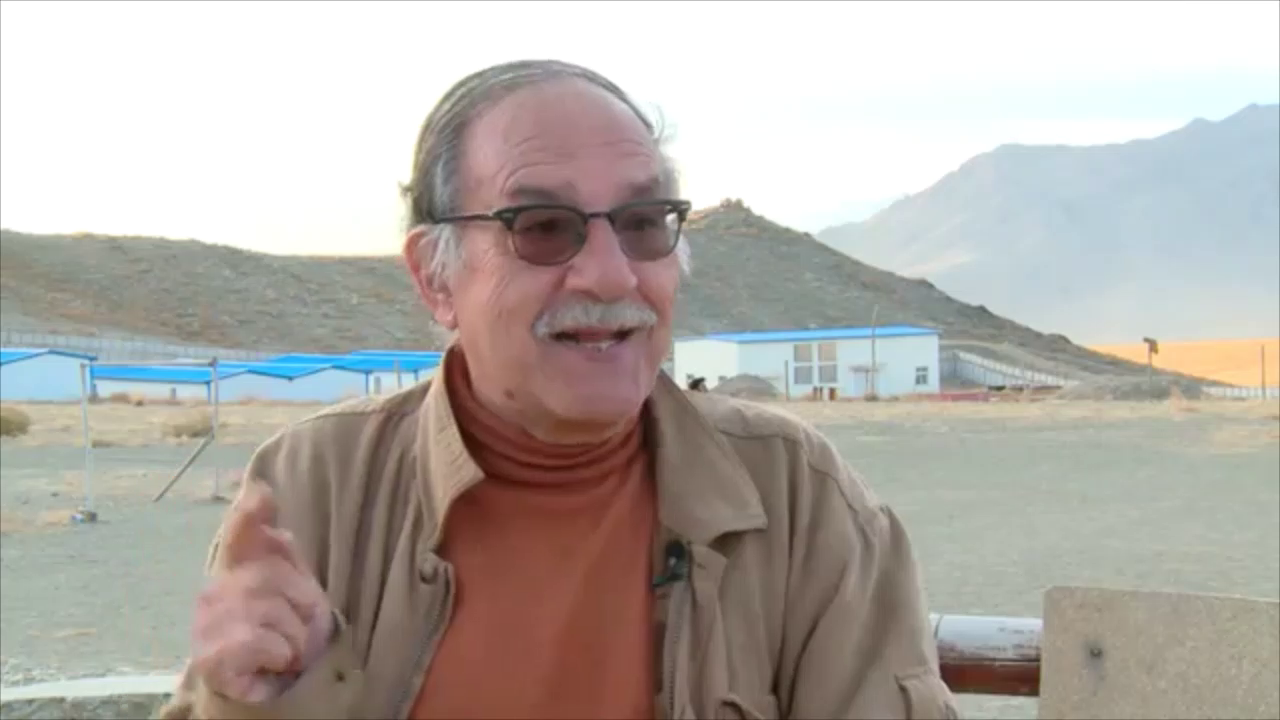
\includegraphics[width=4.2cm]{Figures/mmCult1/frame513.png} 

\end{tabular}
\caption{Cultural level - Example 1}
\begin{footnotesize}
Source: \url{https://www.youtube.com/embed/z6ewpjWYfYo?start=535&end=555}
\end{footnotesize}
\label{fig:figure1}
\end{figure}

The pointing of the finger in the above example functions to accentuate the message. There is a transition from palm up hand open (coinciding with ``with all these wars...''), to hand closed and index finger extended. This gesture transition coincides with emphasis in speech tone. Intonation and pauses with the words ``identity,'' ``culture,'' and ``comes'' further add emphasis. The pointing can also be an indication of high confidence in the message. In the previous ecological level excerpts, we mainly observe examples of iconic gestures that closely reflect the literal meaning of the speech. Here, we begin to see more metaphoric gestures that depict abstract ideas \citep[66]{Beattie2016}. For example, the sweeping motion to describe decades of wars is a metaphoric evocation of the passage of time. The pointing might also be interpreted as a metaphoric reference. Whereas pointing is typically a gesture used for object individuation \citep[115]{Kendon2003}, in this example it is used to `point to' the main concept in the message; namely culture and identity.      

In the next example, the video frame does not include hand gestures. However, there are subtle head movements and facial expressions. In this segment, the speaker is addressing the issue of a proposed mine near ancient burial sites. 

\textbf{\underline{Cultural Level - Example 2}}

\begin{footnotesize}
\texttt{(It's) [my prehistoric ancestors]\textsuperscript{1} (.) that are right within this mining area and [I don't want (.) .hhh hhh you know]\textsuperscript{2} [any \annotate{mine}]\textsuperscript{3} near them, >I don't want any equipment near them.< We have <three known \annotate{burial}> (mound) groups that are there.} 
\end{footnotesize}

\begin{footnotesize}
\begin{enumerate}
    \item Nodding head on beat
   \item Shaking head
   \item Left lip tightened and raised; slight raising of shoulders
\end{enumerate}
\end{footnotesize}

\begin{figure}[H]
\centering
\begin{tabular}{llll}
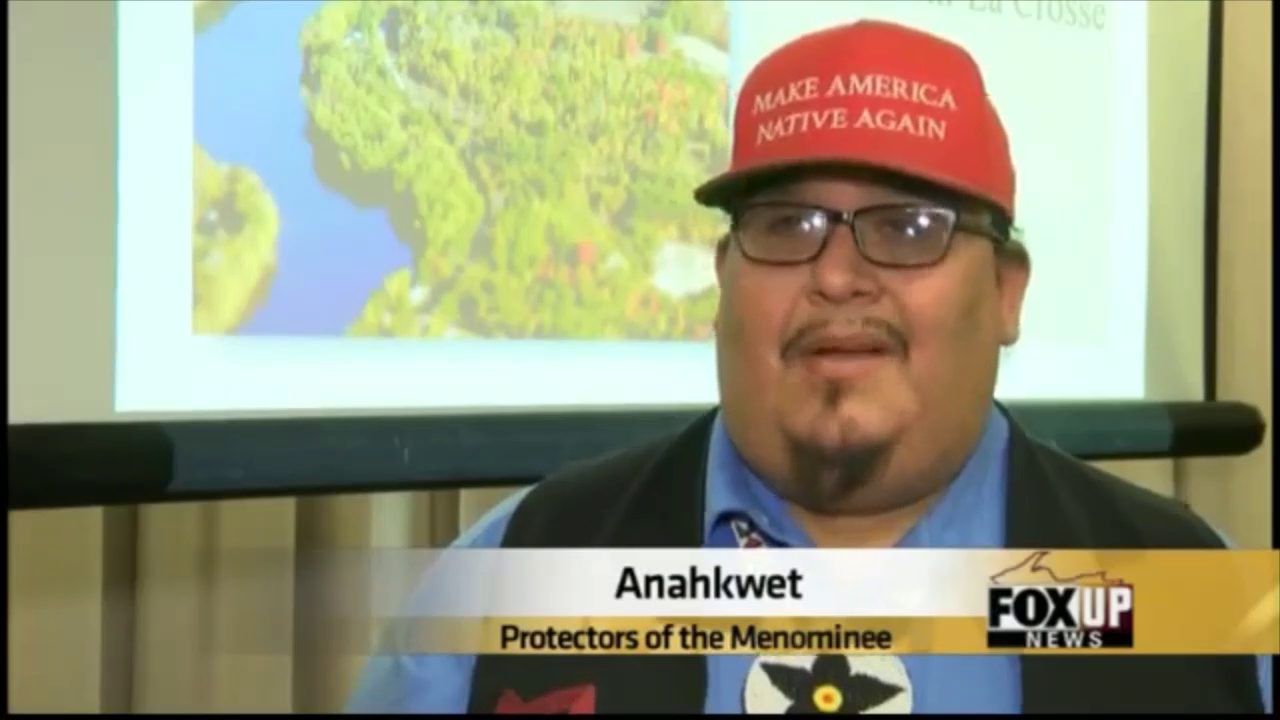
\includegraphics[width=4.2cm]{Figures/mmCult2/frame202.png} & 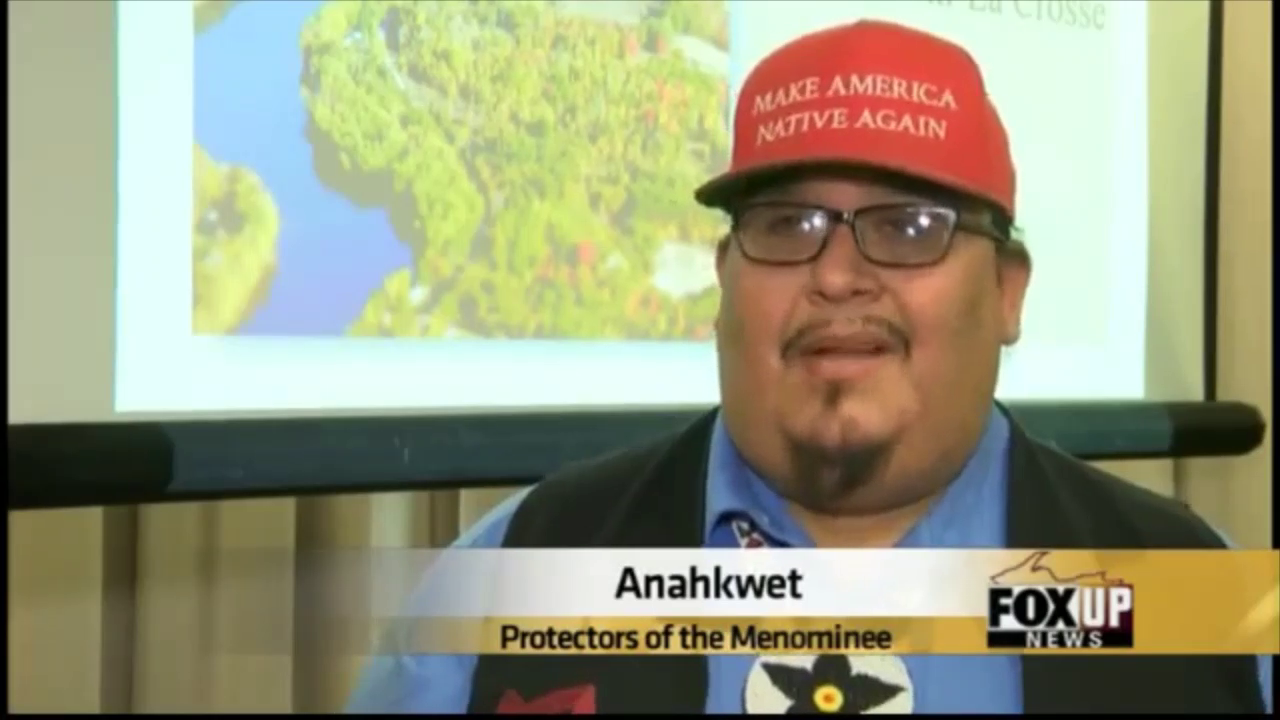
\includegraphics[width=4.2cm]{Figures/mmCult2/frame203.png} & 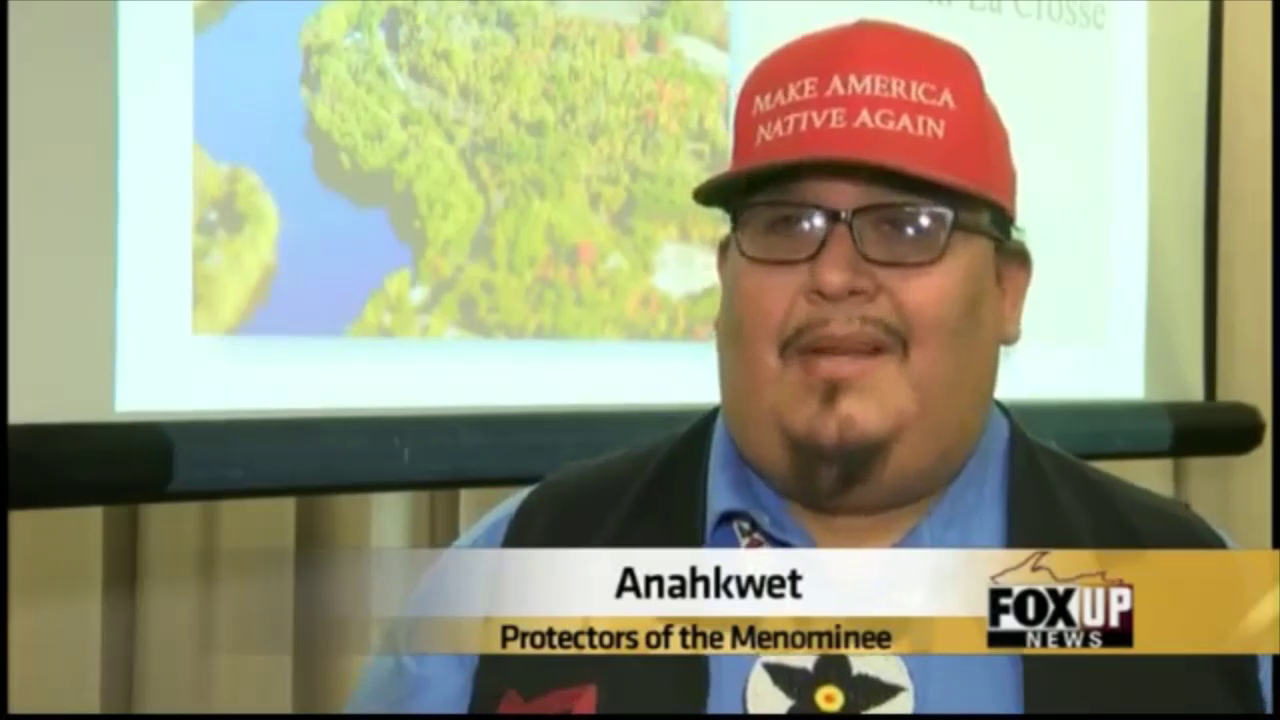
\includegraphics[width=4.2cm]{Figures/mmCult2/frame204.png} 

\end{tabular}
\caption{Cultural level - Example 2}
\begin{footnotesize}
Source: \url{https://www.youtube.com/embed/10FrfEa0Xck?start=33&end=45}
\end{footnotesize}
\label{fig:figure1}
\end{figure}

The head movements of nodding and shaking express emphasis and disapproval, respectively. The brief facial expression near the words ``any mine'' carries a high degree of emotional information. At this point, the corner of the lip is tightened and slightly raised. This expression is the topic of some of the earliest studies of body language. It is what \cite*{Darwin1872} described as ``the upper lip being retracted in such a manner that the canine tooth on one side of the face alone is shown'' (249-250). This was seen by Darwin as an expression inherent to both human and non-human animals when facing an antagonist. Sometimes referred to as a ``sneer,'' it's been suggested that this expression is a universal (cross-cultural) sign of contempt \citep{Izard1988}.

Elements of paralanguage are also observed in this segment. Stress is placed on the words \textit{mine} and \textit{burial}. There is also an audible inhale/exhale immediately before the contempt expression discussed above.  Altered breathing patterns can be indicative of agitation and emotional strain, including the anticipating of anger \citep[118]{Poyatos2002a}.

Example 3 below also relates to mining development on sacred indigenous grounds. Here, the hands, head, and eyes combine to form a cluster of nonverbals depicting the emotional context.

\textbf{\underline{Cultural Level - Example 3}}

\begin{footnotesize}
\texttt{<[They crushed out sacred site]>.\textsuperscript{1} They never [listened to aboriginal people, <elders, female elders>]\textsuperscript{2} (.) you know they've been [\annotate{stomped} on].\textsuperscript{3} So it's time for them to \annotate{stand} up and say [hey you're not doing this to me anymore].\textsuperscript{4}} 
\end{footnotesize}

\begin{footnotesize}
\begin{enumerate}
   \item Right hand motion forward on beat; palm up; index finger and thumb touching
   \item Right hand motion forward on beat; palm up; fingers and thumb open; high blink rate
   \item Head swipe, left to right with emphasis
   \item Head motion with clenched fist
\end{enumerate}
\end{footnotesize}

\begin{figure}[H]
\centering
\begin{tabular}{llll}

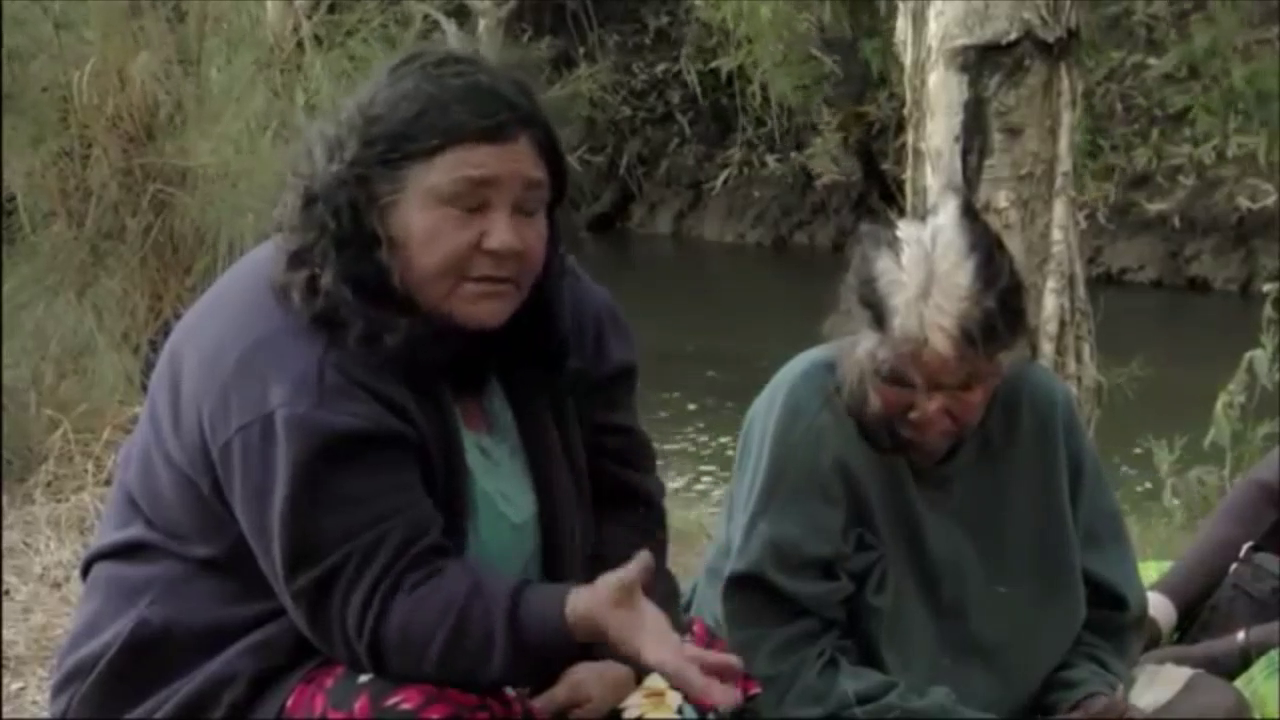
\includegraphics[width=4.2cm]{Figures/mmCult3/frame85.png} & 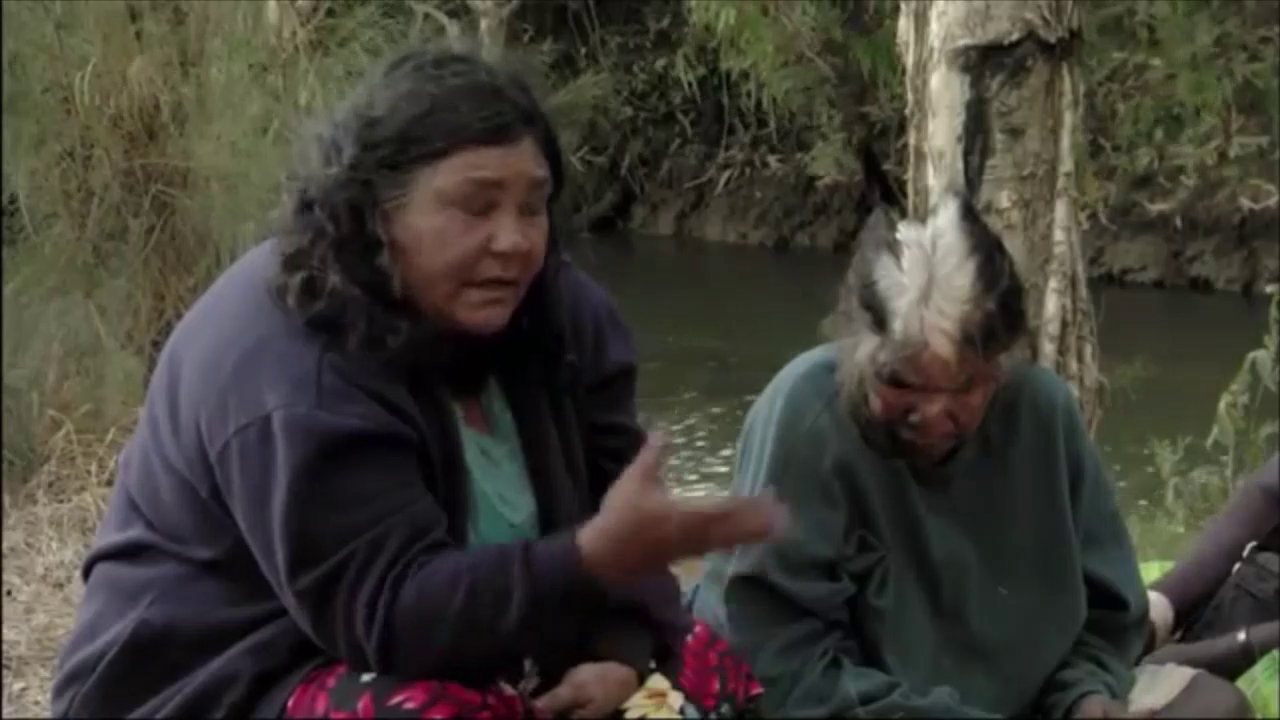
\includegraphics[width=4.2cm]{Figures/mmCult3/frame128.png} & 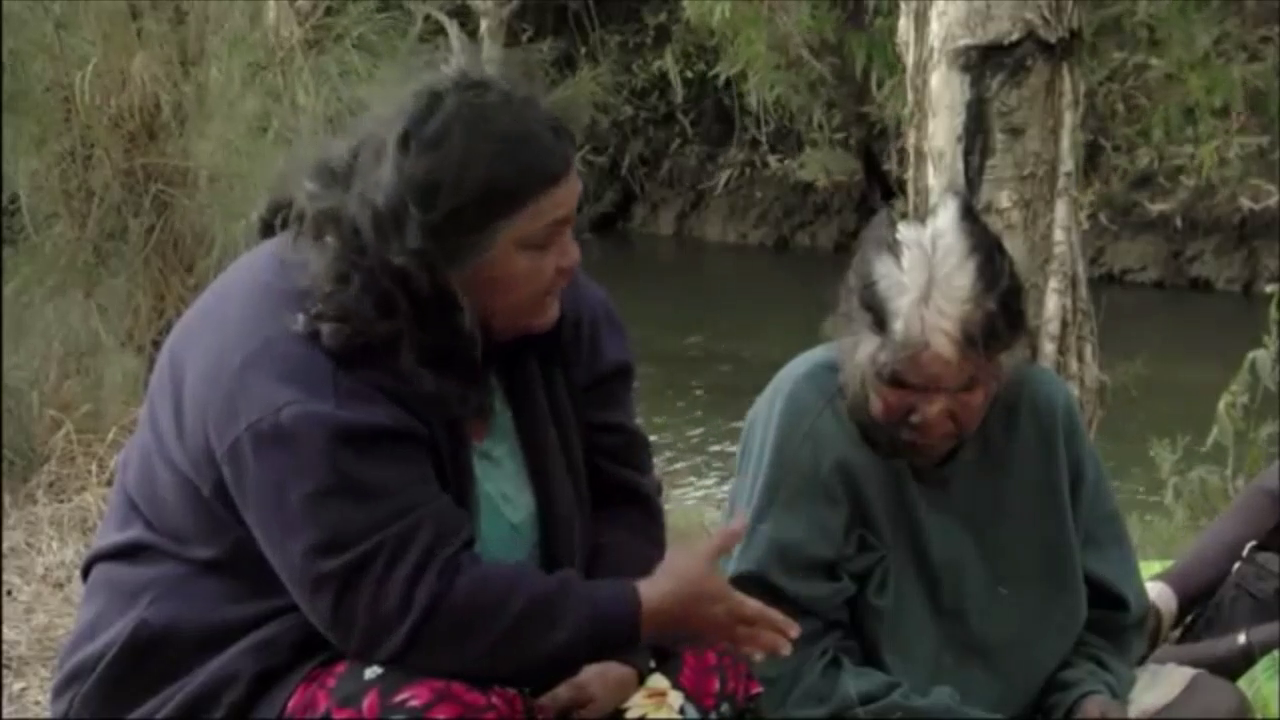
\includegraphics[width=4.2cm]{Figures/mmCult3/frame141.png}  

\end{tabular}
\caption{Cultural Level - Example 3}
\begin{footnotesize}
Source: \url{https://www.youtube.com/embed/awnLI4pRnUM?start=42&end=58}
\end{footnotesize}
\label{fig:figure1}
\end{figure}

As in previous examples, the on-beat hand movements are emphatic. The speaker clenches her fist when saying the words ``hey you're not doing this to me anymore.'' A clenched fist can be a sign of frustration, annoyance, or stress \citep[104]{Phipps2012}. It can also be interpreted as an ``encouragement gesture'' used communicate success or to function in self-encouragement or the encouragement of others \citep{Tops2006}. Here, the fist gesture could function as both an expression of frustration and affirmation to fight back. 

Also notable in Example 3 are the eyes and facial expressions. Around the words ``elders...female elders'' we observe a relatively high blink frequency and duration.  High blink rate (or lower blink inhibition) has been correlated to negative emotional states including stress \citep{Haak2019} and fear \citep{Maffei2019}. The speaker also displays narrowed eyes and a furrowed forehead, both strong indicators of negative emotions.

The context of the next excerpt, Example 4, is drinking water contamination due to mountain top coal mining. This is included in the cultural-level due to the religious sentiments expressed. As in the previous example, both hand and eye movements are telling indicators of emotions. 

\textbf{\underline{Cultural Level - Example 4}}

\begin{footnotesize}
\texttt{You \annotate{pray} before you go to bed... and >you just ask God to protect (you and) your family, that's all you \annotate{can} do,< because (.) [\annotate{man} has done the damage to the earth (.) and man]\textsuperscript{1} (.) [I don't see how <man can correct what's been done>]\textsuperscript{2}. [\annotate{God} can handle this (.) and he will. When the right time comes]\textsuperscript{3}, he will do what needs to be done.}
\end{footnotesize}

\begin{footnotesize}
\begin{enumerate}
   \item Right hand motions forward; palm up
   \item Right hand motions forward, fingers and thumbs curled inward; head shaking
   \item Rand waves outwards, stops at thigh; gaze upwards to sky; nodding 
\end{enumerate}
\end{footnotesize}

\begin{figure}[H]
\centering
\begin{tabular}{llll}


\includegraphics[width=4.2cm]{Figures/mmCult4/frame237.png} & 
\includegraphics[width=4.2cm]{Figures/mmCult4/frame245.png} & 
\includegraphics[width=4.2cm]{Figures/mmCult4/frame437.png}  

\end{tabular}
\caption{Cultural level - Example 4}
\begin{footnotesize}
Source: \url{https://www.youtube.com/embed/UvKe2LYy5pk?start=1198&end=1220}
\end{footnotesize}
\label{fig:figure1}
\end{figure}

Early in the segment, we see an open hand palm up gesture similar to that in previous segments. This is followed by a palm up with hands curled inward and index finger and thumb touching. This quickly transitions into a final wave of the hand and gaze upwards with the words ``God can handle this.'' This sequence of movements is a nonverbal juxtaposition between man and God. The finer detailed, downward hand movements (when talking about man) give way to a more spontaneous, upward motion when evoking the spiritual realm. The gaze also shifts upward when referencing God. The words ``he [God] will do what has to be done...'' are accompanied by affirmative nodding. 

The fifth and final cultural-level example features a coal mining worker responding negatively to protesters. In the previous examples, cultural identity is expressed along national, ethnic, or religious lines. In Example 5, culture is expressed in terms of locality and regional (sub-national) affiliation. 

\textbf{\underline{Cultural Level - Example 5}}

\begin{footnotesize}
\texttt{If [they're for us]\textsuperscript{1}, that's good. If they're [against us, get out]\textsuperscript{2} of the state.}
\end{footnotesize}

\begin{footnotesize}
\begin{enumerate}
   \item Hand motion down towards ground, index finger extended
   \item Thumb up; hand motion back over left shoulder
\end{enumerate}
\end{footnotesize}

\begin{figure}[H]
\centering
\begin{tabular}{llll}

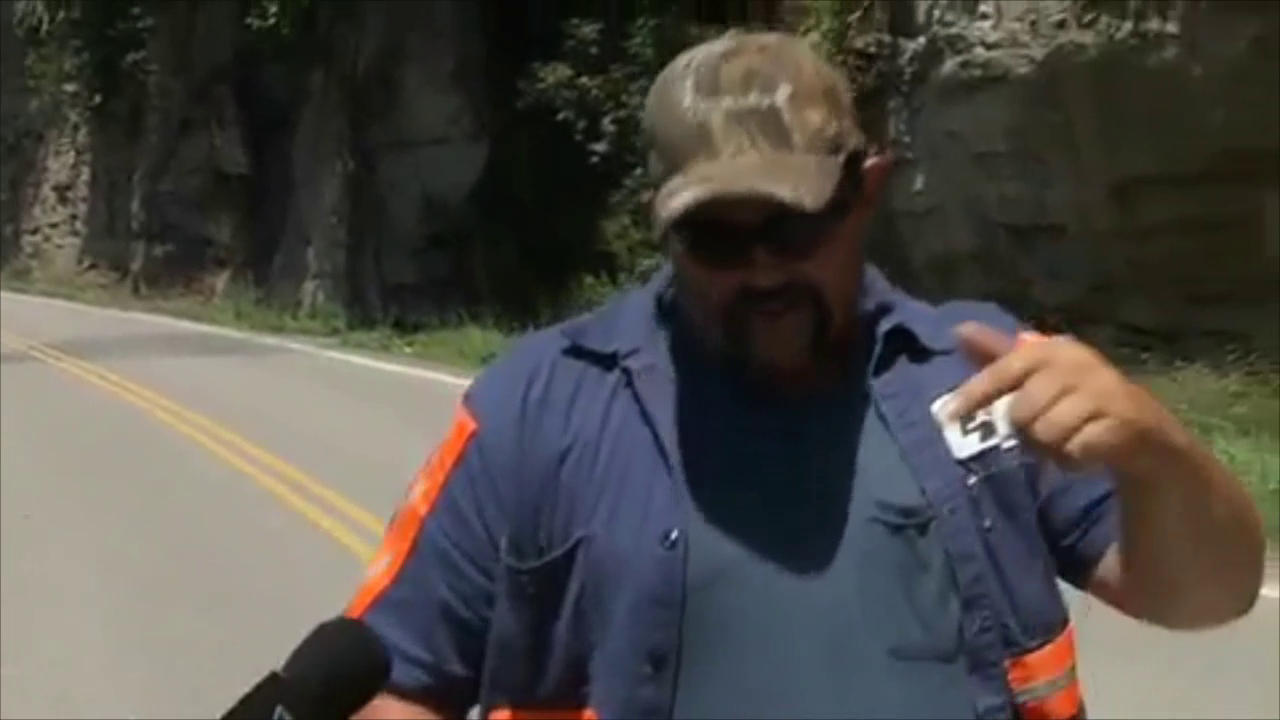
\includegraphics[width=4.2cm]{Figures/mmCult5/frame19.png} & 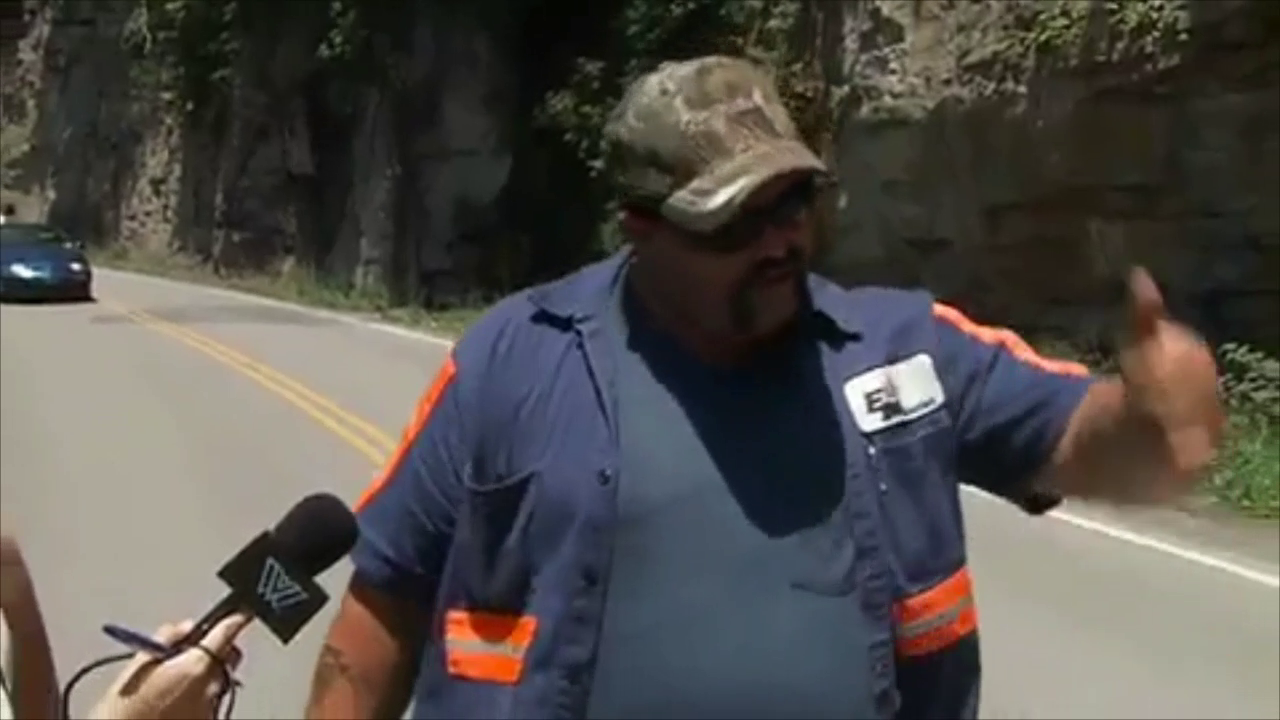
\includegraphics[width=4.2cm]{Figures/mmCult5/frame103.png} & 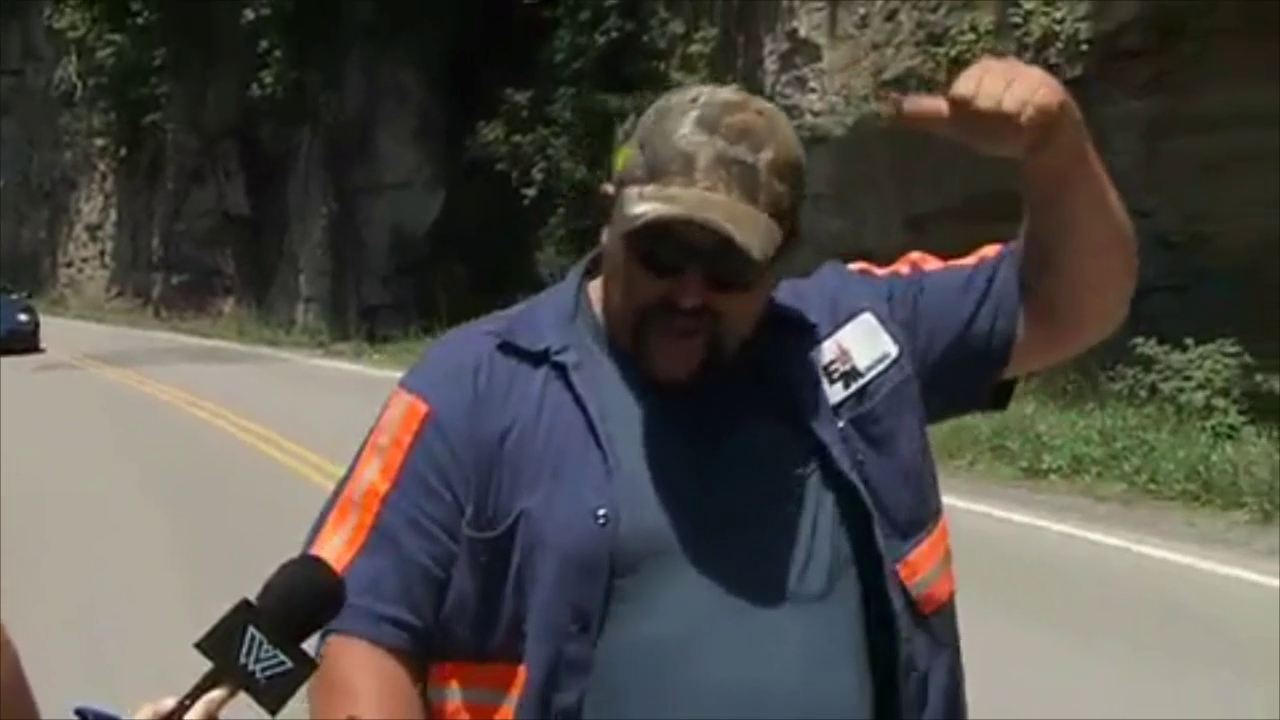
\includegraphics[width=4.2cm]{Figures/mmCult5/frame118.png}  

\end{tabular}
\caption{Cultural Level - Example 5}
\begin{footnotesize}
Source: \url{https://www.youtube.com/embed/vBhvFWRLiOs?start=467&end=476}
\end{footnotesize}
\label{fig:figure1}
\end{figure}

This example shows how in-group/out-group dynamics are embodied in gesture. The words ``if they're for us...'' is accompanied by a pointing downwards in front. When referring to those ``against us,'' the speaker gestures with his thumb over the left shoulder. Using the thumb to point in this way is considered a sign of ridicule and disrespect \citep[140]{Lewis2012}. Thumb displays in general are also associated with expressions of power and authority. Here, the thumb display might be seen as an embodiment of the confidence associated with in-group association.   

\textbf{Summary of Cultural-Level}

What's evident at the cultural-level is an increased animation of nonverbal communication. Hand movements appear more spontaneous and forceful than in the previous, ecological-level examples. Facial expressions and eye movements are also more apparent. The hand movements include markers of emphasis including pointing and on-beat movements. Clenched fist and thumb displays also signal stronger, more emotive communication. Head movements are more pronounced compared to the ecological-level, both through negative shaking and affirmative nodding. Facial expressions include increased blink rates and, in one case, the well known indicator of contempt by raising one side of the lip.   

The cultural-level examples also exhibit a high degree of confidence and affirmation. Pointing, fist clenching, and nodding are signals that speakers believe in their message and affirm it. Similarly, the thumb display in the final example is a high confidence gesture.   

\subsection{Socio-Economic Level}

The socio-economic level features four examples. In these examples, speakers refer to issues of justice, economics, and social institutions. These include a woman speaking about violence surrounding mining projects in Honduras; a woman addressing an audience regarding the need to economic opportunities in their community; a retired miner talking about the lack of institutional regulation towards the coal industry; and a woman stressing the importance of coal mining to her families' livelihood.

Example 1 below is a segment from an interview with a Lenca indigenous woman in Honduras. 

\textbf{\underline{Socio-Economic Level - Example 1}}

\begin{footnotesize}
\texttt{(Translated from Spanish - only gesture annotation)
The worst impacts have been state violence. Why? Because we have comrades who have been killed following military harassment. [We've already lost one person].\textsuperscript{1}}
\end{footnotesize}

\begin{footnotesize}
\begin{enumerate}
   \item Raised eyebrows; wide eyes; extenuated blinks
\end{enumerate}
\end{footnotesize}

\begin{figure}[H]
\centering
\begin{tabular}{llll}
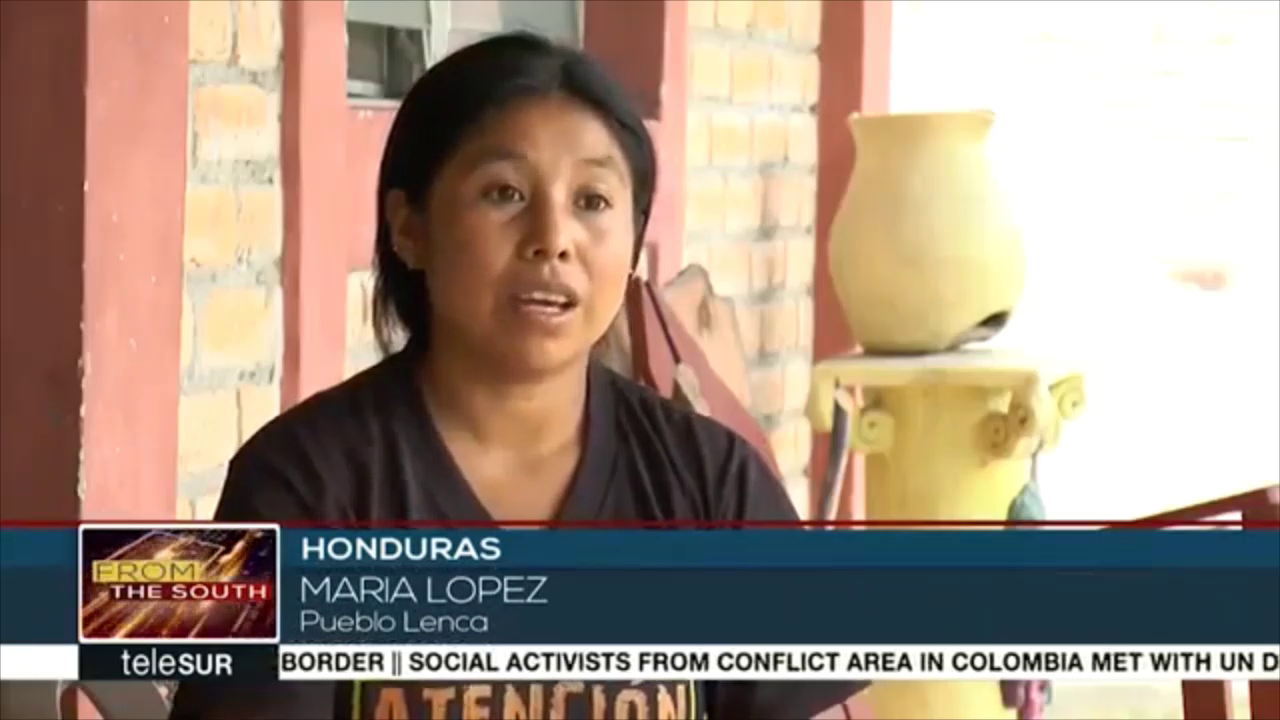
\includegraphics[width=4.2cm]{Figures/mmEcon/frame66.png} & 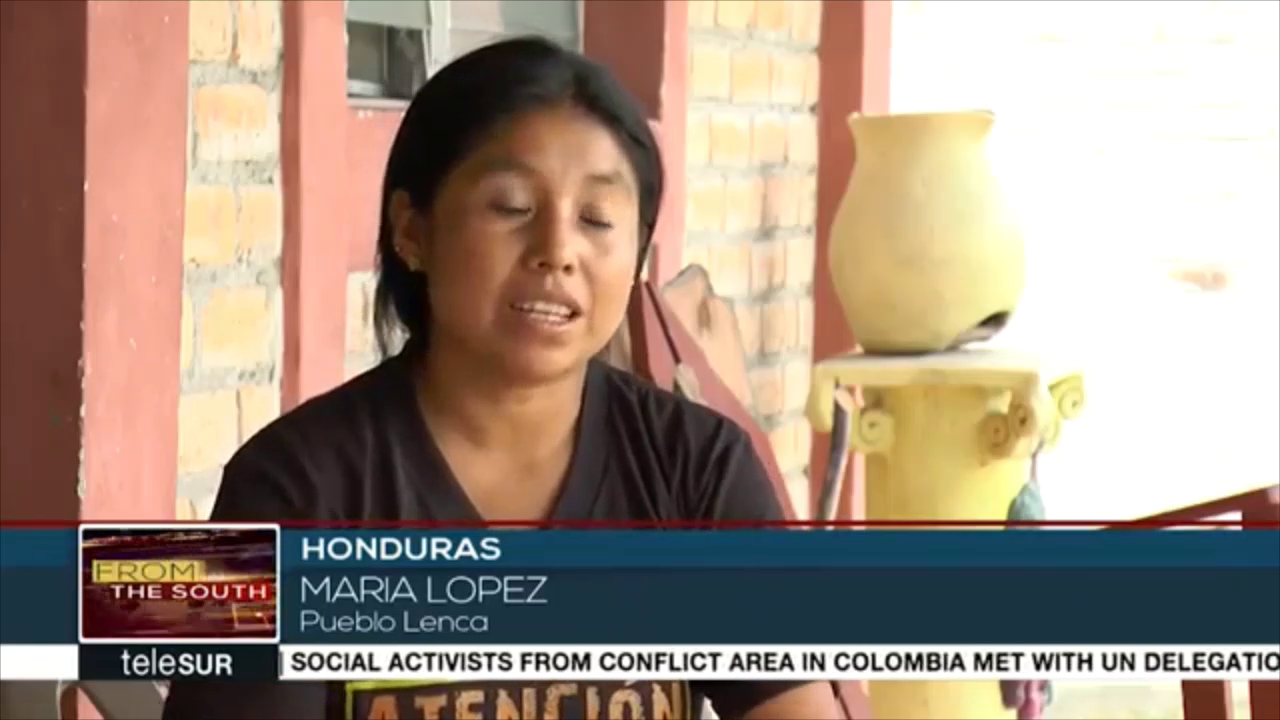
\includegraphics[width=4.2cm]{Figures/mmEcon/frame110.png} & 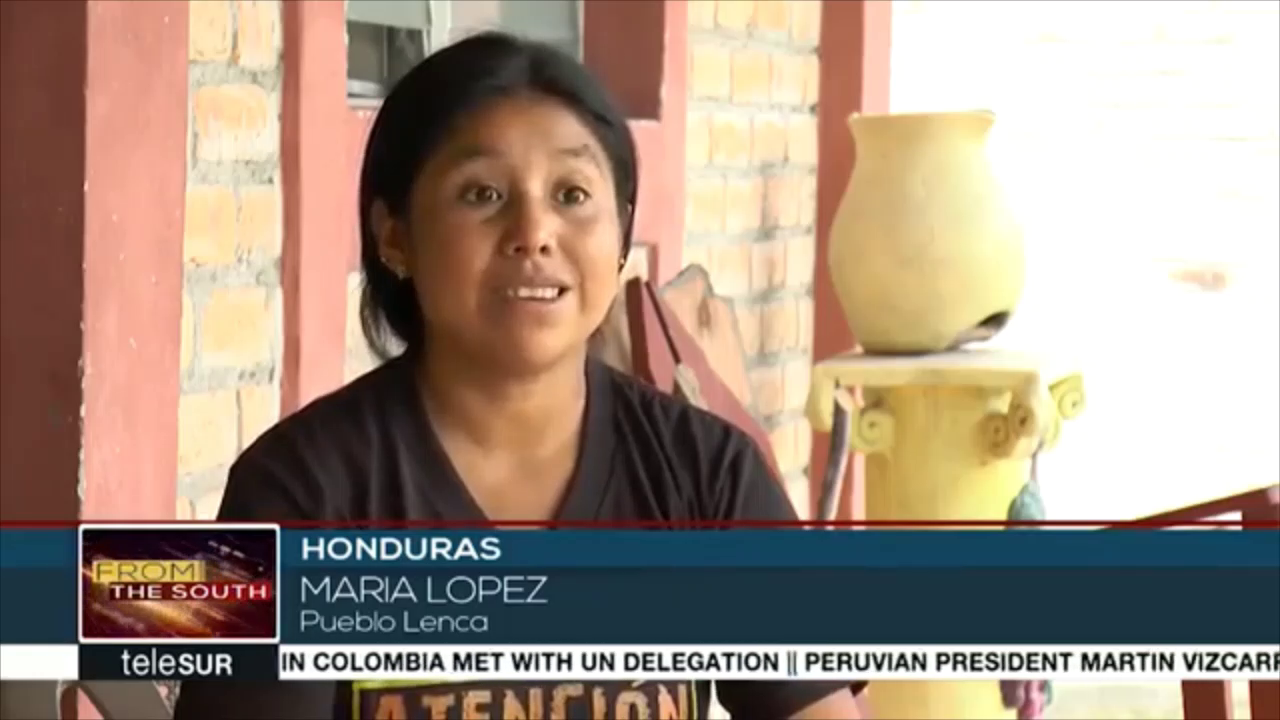
\includegraphics[width=4.2cm]{Figures/mmEcon/frame304.png}  
\end{tabular}
\caption{Socio-Economic level - Example 1}
\begin{footnotesize}
Source: \url{https://www.youtube.com/embed/gU7PBoy-wFE?start=10&end=21}
\end{footnotesize}
\label{fig:figure1}
\end{figure}

In this example, the analysis is largely limited to facial expressions. As she discusses violence and harassment from mining and hydroelectric projects, the eyes and face are strong nonverbal indicators. Particularly in the final frames, the eyebrows are pulled up and together and the eyed widened. The raised eyebrows are characteristic of what's often claimed as a universal facial expression denoting fear \citep[28-30]{Matsumoto2013}. 

Example 2 is unique in that we are able to view body language of listeners as well as the speaker. In this clip a woman is talking about economic hardships in the community in the context of a debate around proposed uranium mining. 

\textbf{\underline{Socio-Economic Level - Example 2}}

\begin{footnotesize}

\texttt{<\annotate{Five years} we'e been trying to keep our doors open, \annotate{thinking} (.) any day now> those jobs were going to be here. >These are the only people that have come in and offered us jobs$\uparrow$< If \annotate{any} of the people here who are against it had come in and [said they had jobs to match it, we'd be behind that too. But right now this is all we've got]\textsuperscript{1}. Everyone one of you who has stood up against this could have brought in jobs [for \annotate{us}.]\textsuperscript{2}}
\end{footnotesize}

\begin{footnotesize}
\begin{enumerate}
   \item Raised and upward slanted eyebrows, stressed blink
   \item Hand points inwards toward chest; index finger extended
\end{enumerate}
\end{footnotesize}

\begin{figure}[H]
\centering
\begin{tabular}{llll}
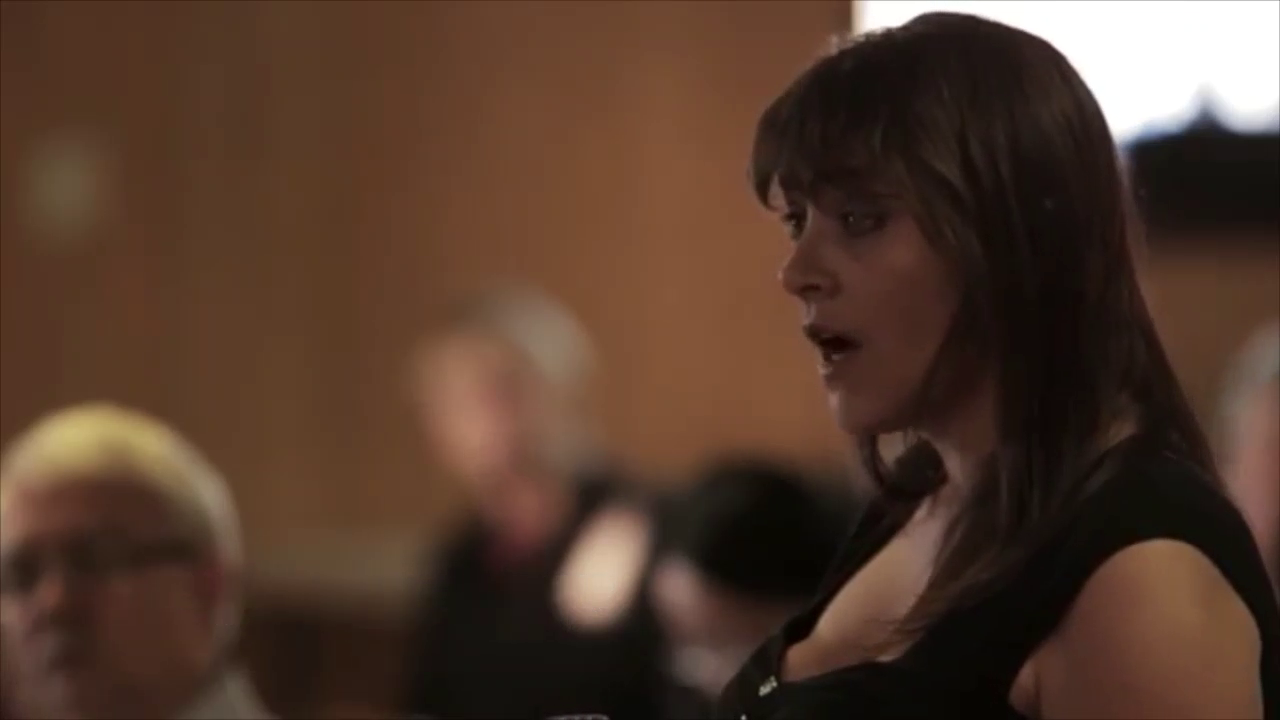
\includegraphics[width=4.2cm]{Figures/mmEcon1/frame413.png} & 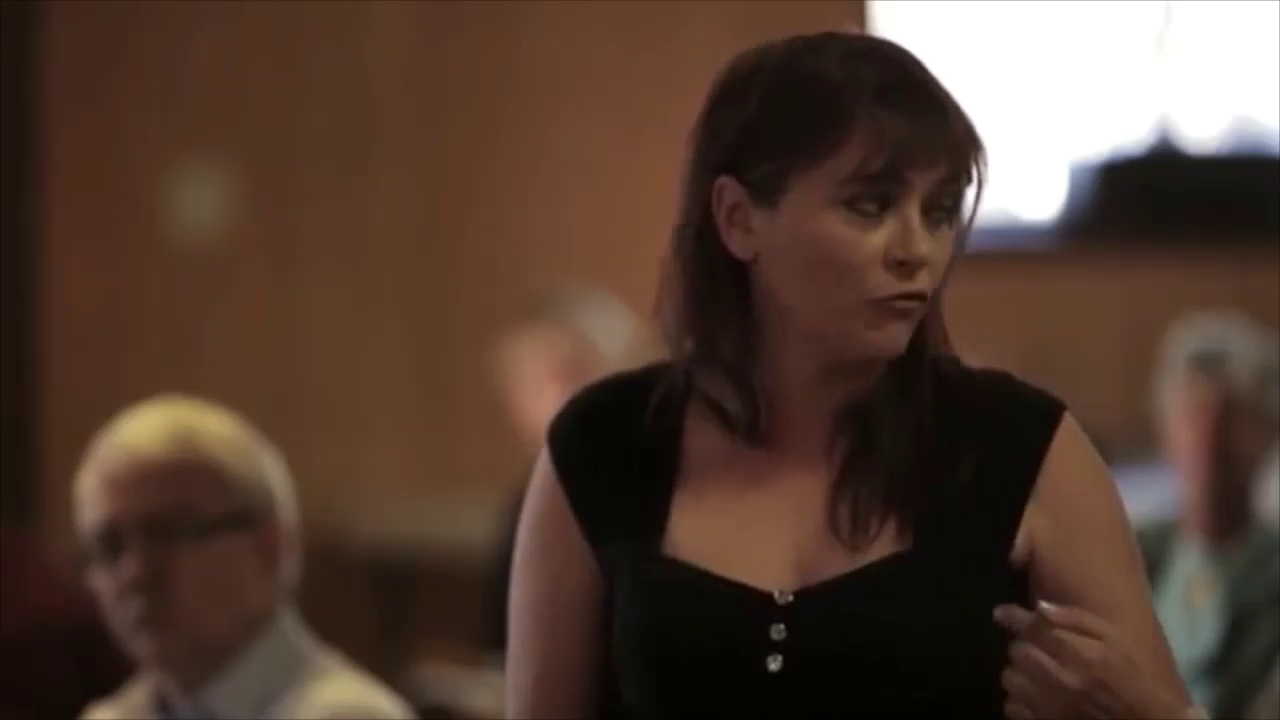
\includegraphics[width=4.2cm]{Figures/mmEcon1/frame725.png} & 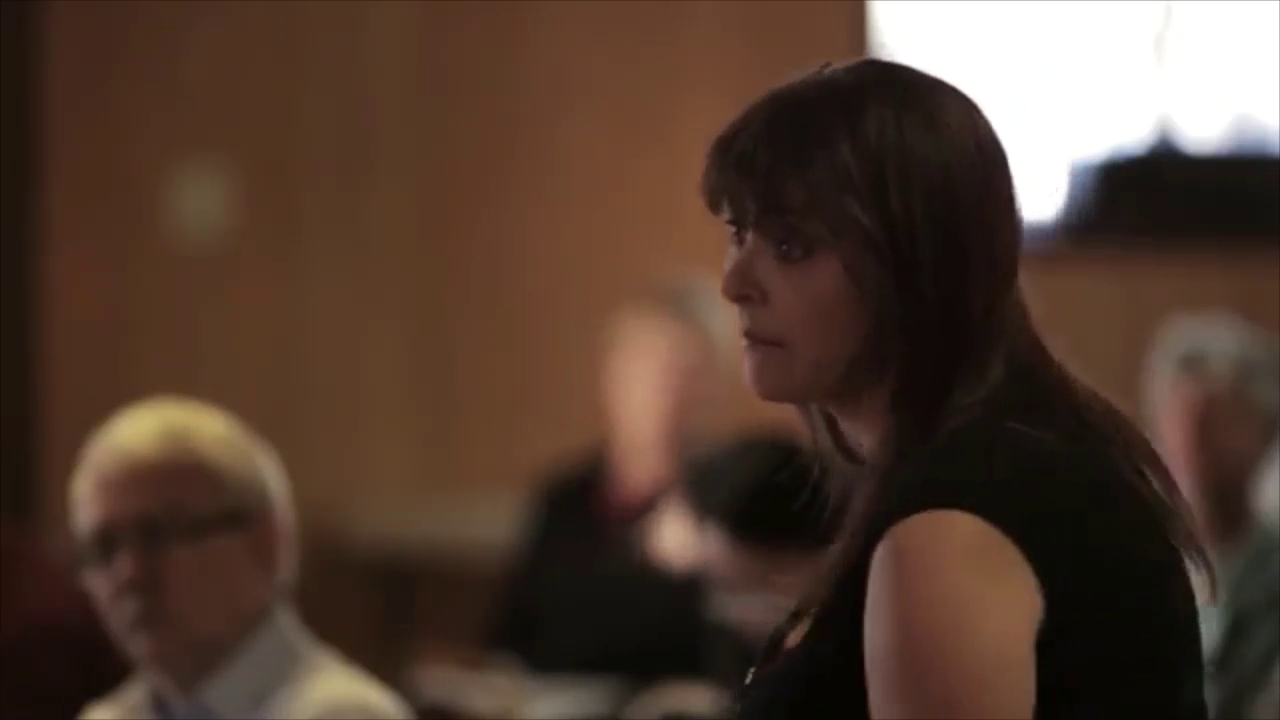
\includegraphics[width=4.2cm]{Figures/mmEcon1/frame988.png}  
\end{tabular}
\caption{Socio-Economic level - Example 2}
\begin{footnotesize}
Source: \url{https://www.youtube.com/embed/Sh0_Wf8F4RM?start=390&end=420}
\end{footnotesize}
\label{fig:figure1}
\end{figure}

\begin{figure}[H]
\centering
\begin{tabular}{llll}
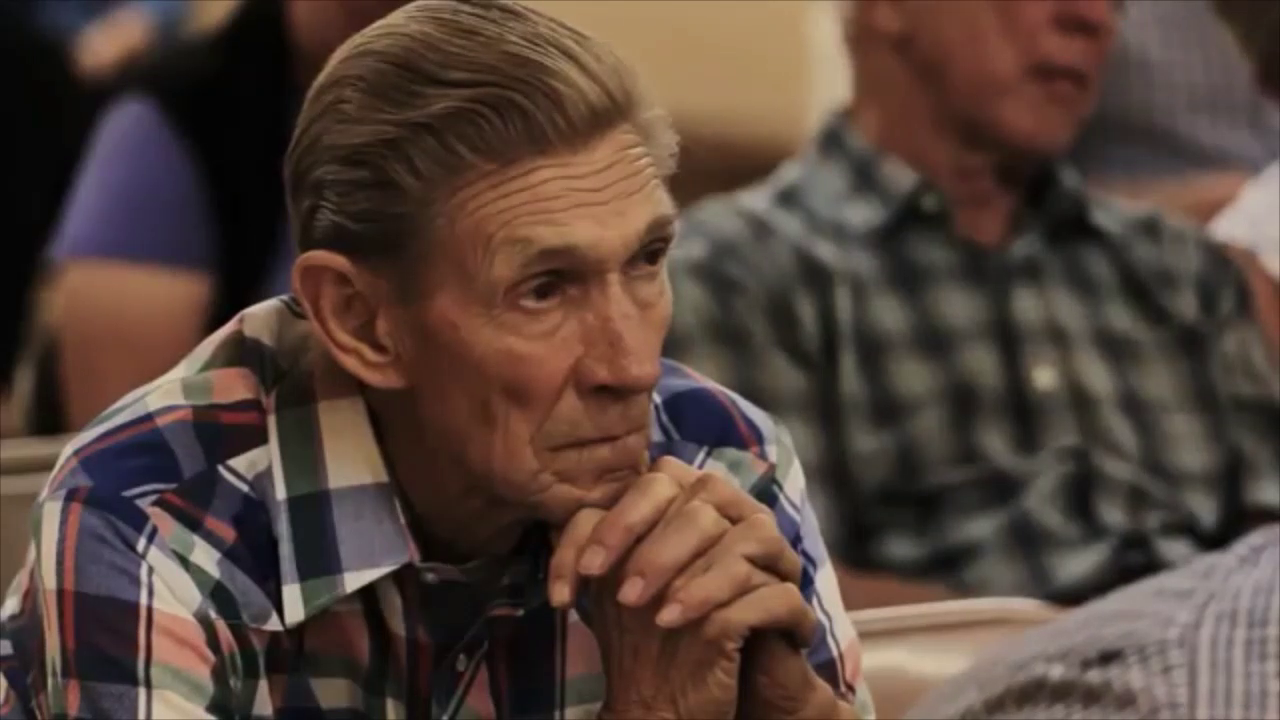
\includegraphics[width=5cm]{Figures/mmEcon2/frame137.png} &  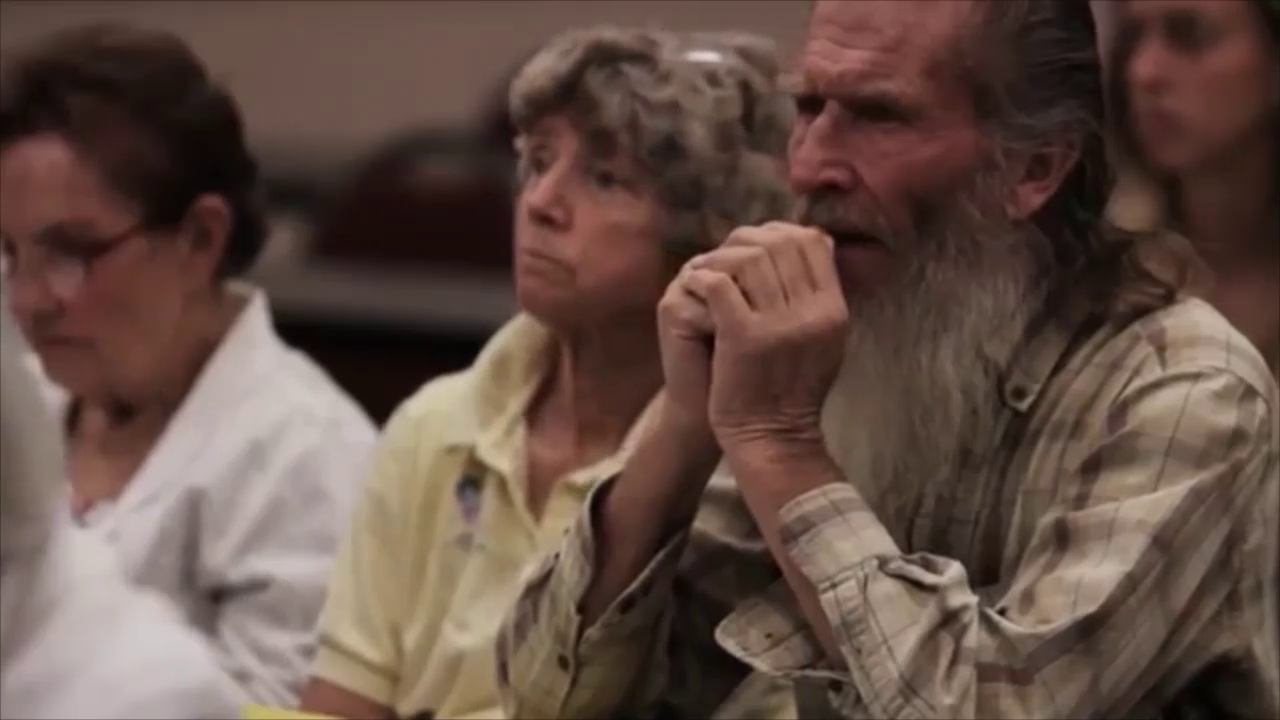
\includegraphics[width=5cm]{Figures/mmEcon2/frame222.png} \\

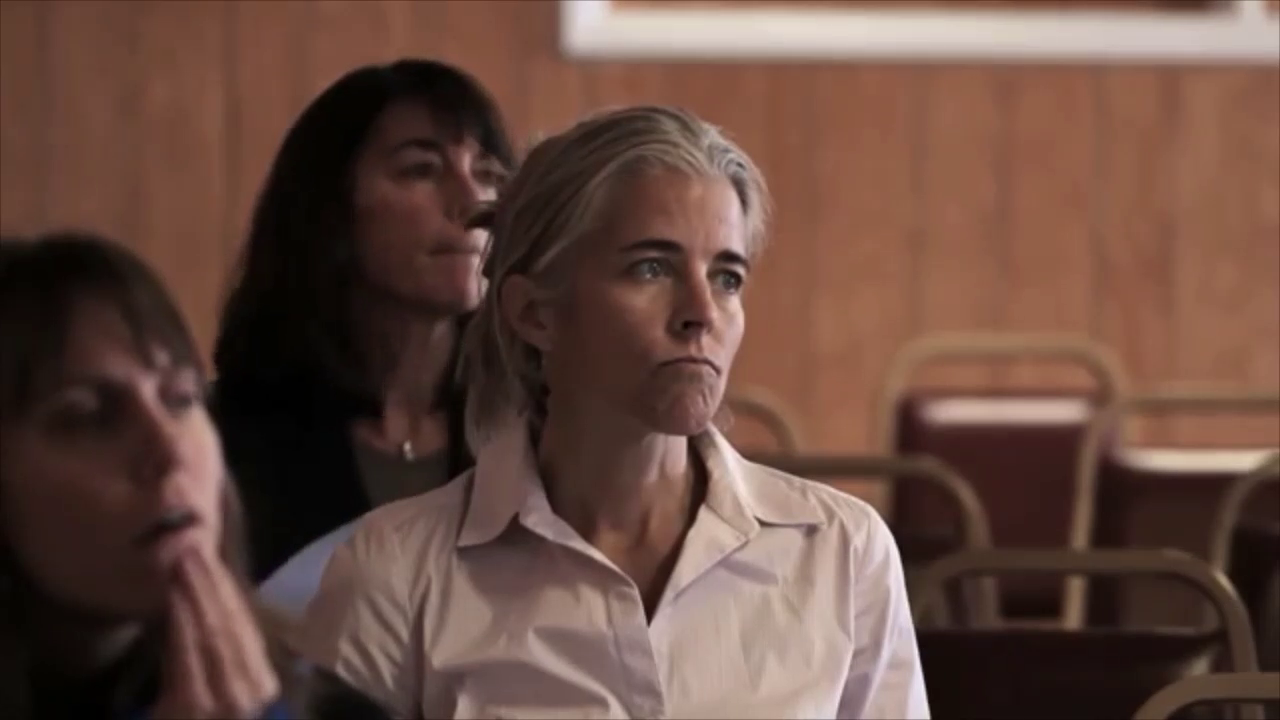
\includegraphics[width=5cm]{Figures/mmEcon2/frame529.png} & 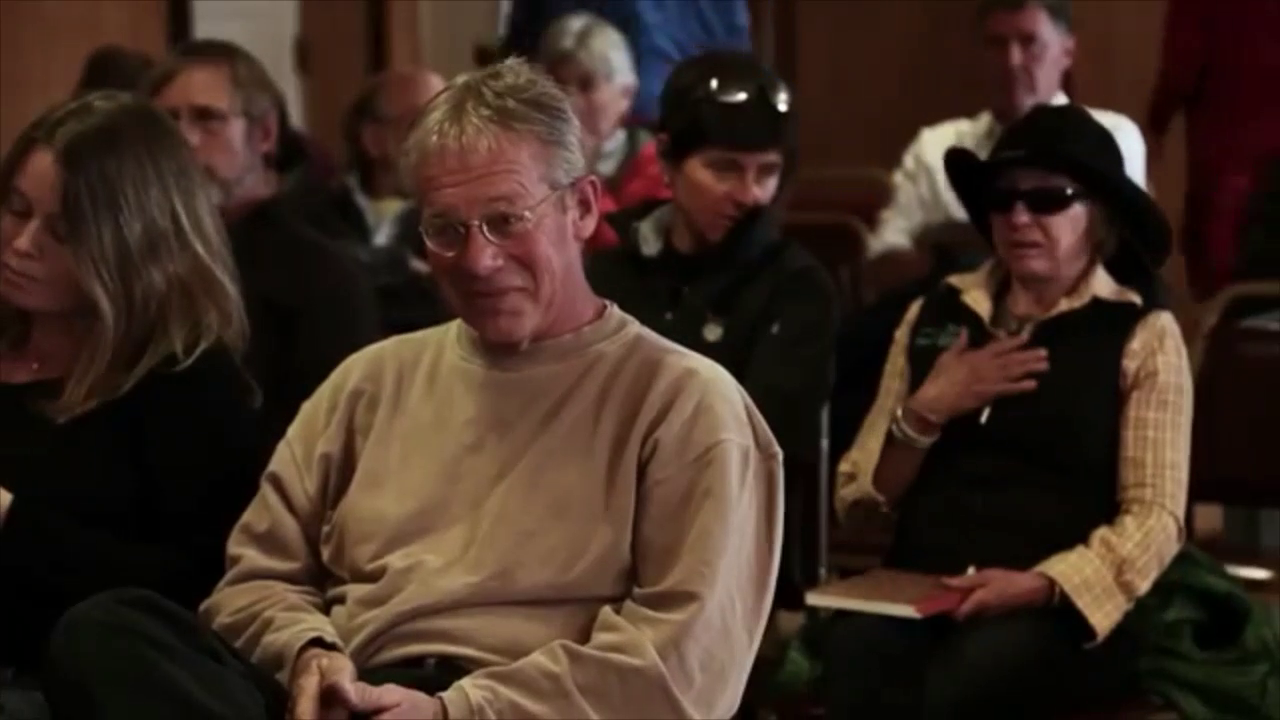
\includegraphics[width=5cm]{Figures/mmEcon2/frame857.png}  

\end{tabular}
\caption{Socio-economic level, listener reactions}
\label{fig:figure1}
\end{figure}

Here we observe an extended blink as well as upward slanted eyebrows. The eyes in particular show concern, worry, and sadness. These expressions are mirrored among listeners. In Figure 5.12 (bottom left) we see a woman with a similar worried and sad expression along with pursed lips. The emotional intensity is apparent given that tearing eyes can be observed, both in the speaker and one of the audience members. Audience members are shown with their hands clenched in front of their faces (Figure 5.12, top left and top right), another indicator of a negative or anxious attitude. On the bottom right of Figure 5.12, we see a man with an obvious expression of sadness as well as a woman behind him with her hand placed on the sternum, a nonverbal expression of empathy.

In this segment, stress and intonation are used more emphatically than in any of the previous segments. For example, in the beginning of the segment, the stress on ``five years'' emphasizes the time duration of hardship. The intonation in the second sentence also conveys a sense of urgency and exasperation. Finally, the stress on the word ``us,'' together with pointing towards the chest, indicates the personal feelings and emotions at play. 

The next example is an interview with a former coal miner on the topic of mountain top removal coal mining.

\textbf{\underline{Socio-Economic Level - Example 3}}

\begin{footnotesize}
\texttt{[They're fighting]\textsuperscript{1} a losing battle I feel (.) myself I feel like they're just fighting a losing battle, because the <[\annotate{politicians}]\textsuperscript{2} and the [\annotate{big} coal companies and things> \annotate{they're} going to win hands down >because the judges and arbitrators are just going to go their way.<]\textsuperscript{3} }
\end{footnotesize}

\begin{footnotesize}
\begin{enumerate}
   \item Both hands extend outward, palms up
   \item Both hands motion forward/downward, palms down
   \item Both hands extend outward, palms up, with emphasis
\end{enumerate}
\end{footnotesize}

\begin{figure}[H]
\centering
\begin{tabular}{llll}
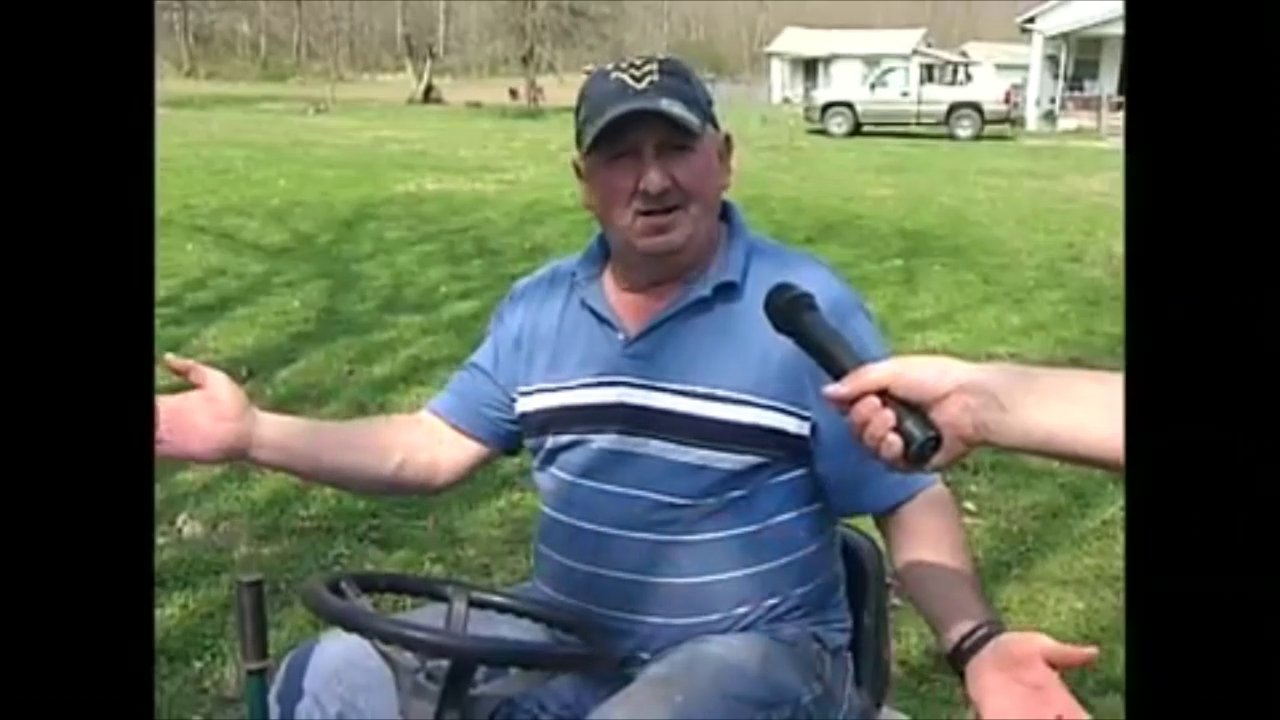
\includegraphics[width=4.2cm]{Figures/mmEcon3/frame189.png} & 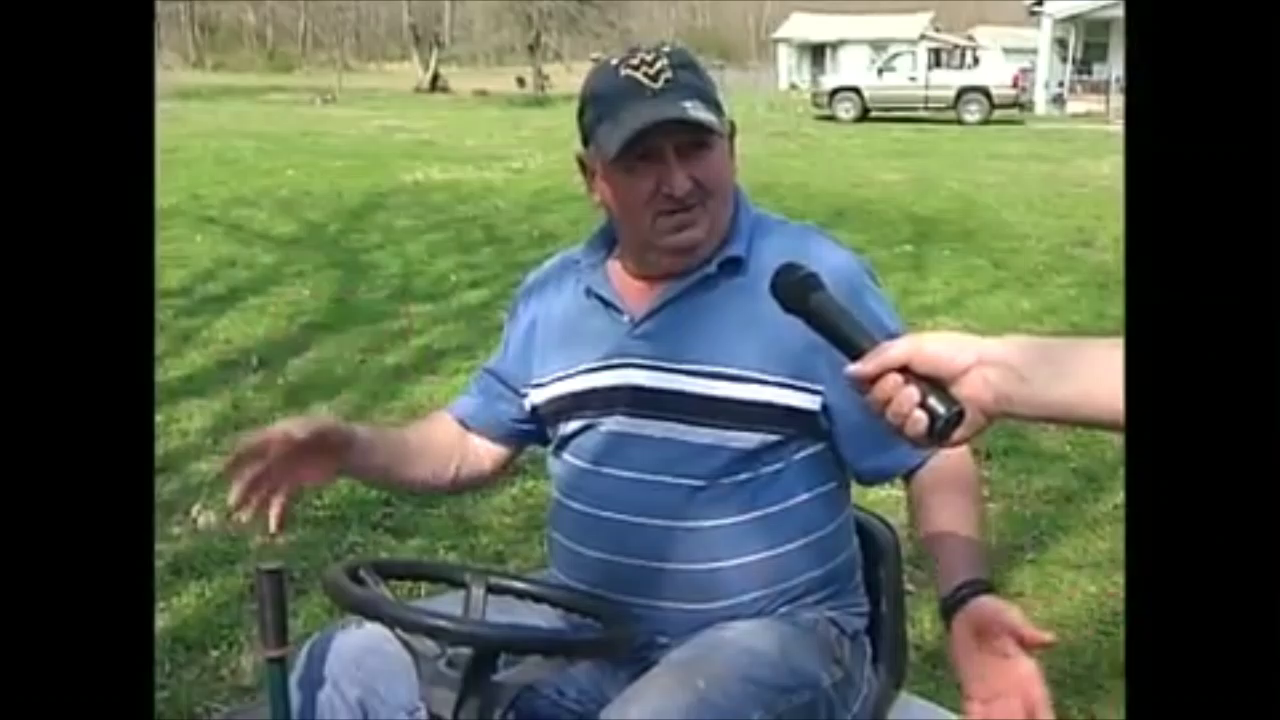
\includegraphics[width=4.2cm]{Figures/mmEcon3/frame450.png} & 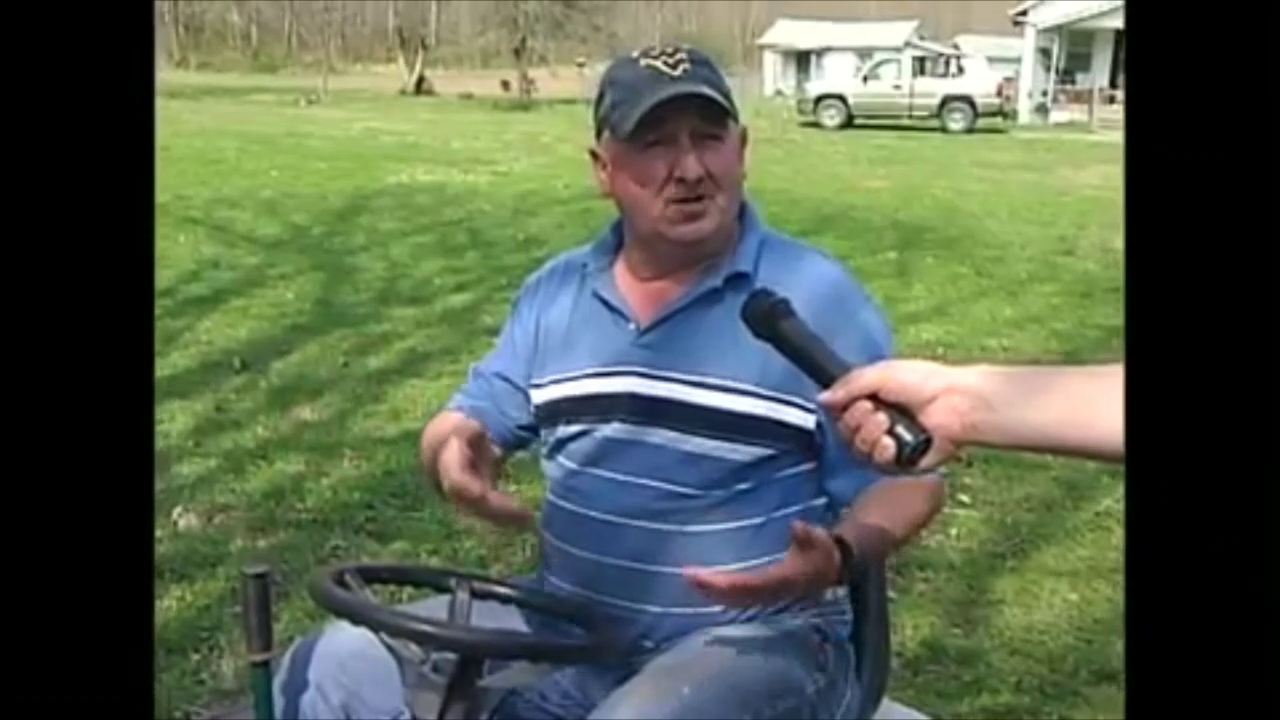
\includegraphics[width=4.2cm]{Figures/mmEcon3/frame610.png}  
\end{tabular}
\caption{Socio-Economic Level - Example 3}
\begin{footnotesize}
Source: \url{https://www.youtube.com/embed/vBhvFWRLiOs?start=1299&end=1316}
\end{footnotesize}
\label{fig:figure1}
\end{figure}

Example 3 exhibits the open hand palm up gesture at various points. At the beginning of the segment the speaker displays an open hands gesture. This open-palm gesture, commonly referred to as a ``pleading'' or ``begging'' gesture \citep[149]{Lewis2012}, depicts a sense of helplessness and resignation. The words ``fighting a losing battle'' complement this sense. The palms-open gesture repeats several times on the stressed words, adding to the sense of futility the speaker is conveying. Briefly, the palm shifts downward to stress the word ``politicians,'' indicating that the speaker is making a strong, assertive point. However, the palms quickly shift upwards for the remainder of the segment. Looking to the facial expressions, we can see eyebrows pinched at the center and sloping downwards. This ``knit brow'' can be interpreted as an expression of worry or concern \citep{Hartley2017}.

The final example is from the same piece on mountain top removal coal mining. The speaker is defending the coal miners and stressing the importance of the industry for her community and family.

\textbf{\underline{Socio-Economic Level - Example 4}}

\begin{footnotesize}
\texttt{If you choose to live in West Virginia, [this is (.) this is the best paying job there is$\uparrow$]\textsuperscript{1}. \textit{Interviewer}: What happens if mountain top removal goes away, what happens to you and your family? \annotate{WE GO HUNGRY!}\textsuperscript{2}}

\end{footnotesize}

\begin{footnotesize}
\begin{enumerate}
   \item Shoulders raise; nodding
   \item Eyebrows raise
\end{enumerate}
\end{footnotesize}

\begin{figure}[H]
\centering
\begin{tabular}{llll}
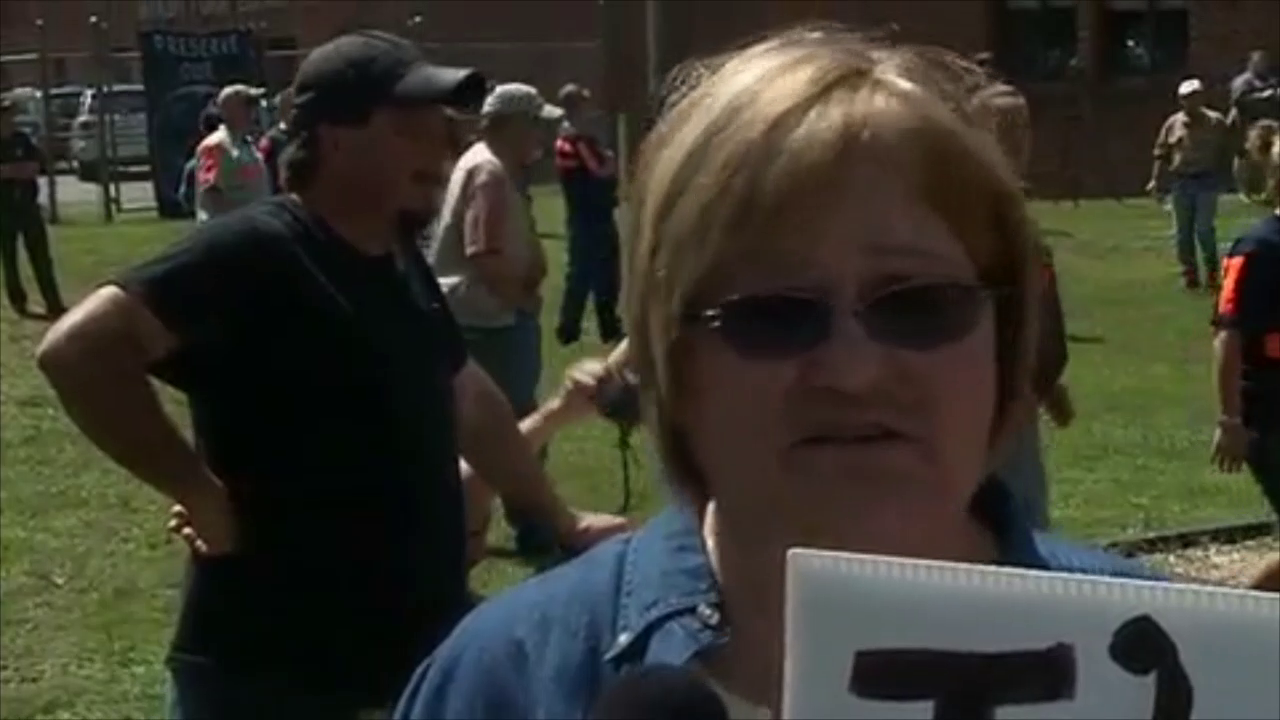
\includegraphics[width=4.2cm]{Figures/mmEcon4/frame3.png} & 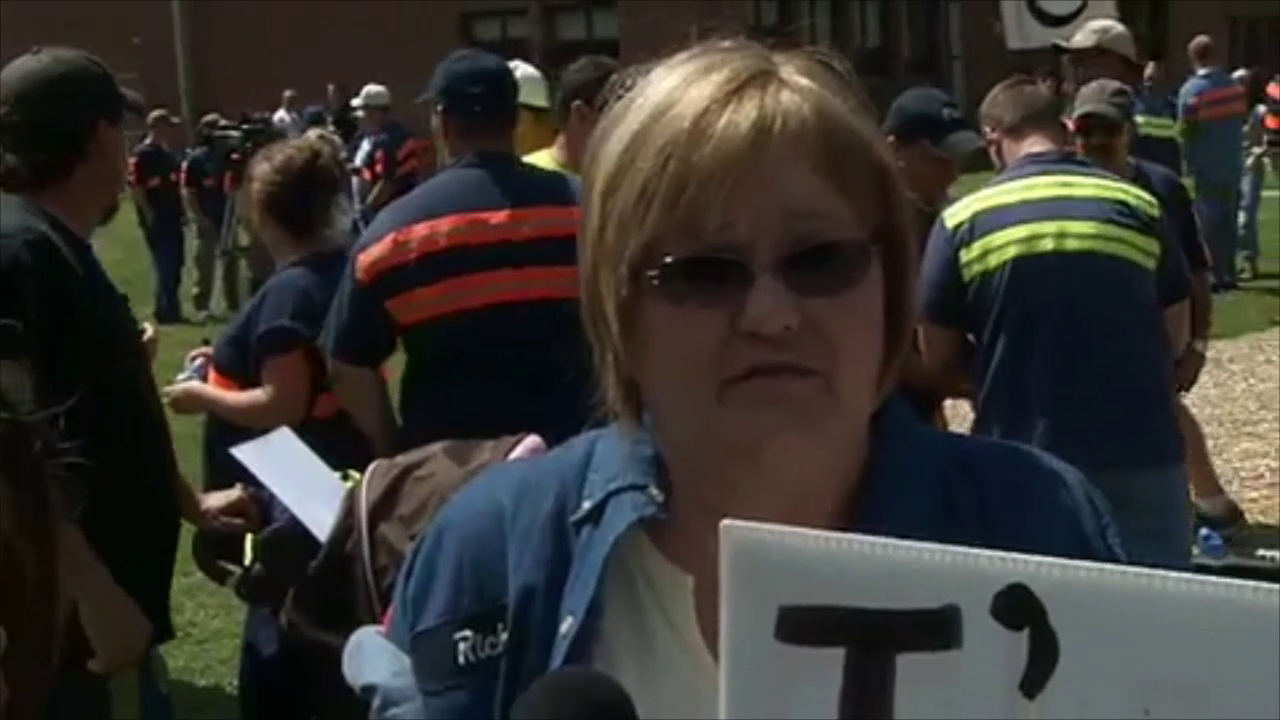
\includegraphics[width=4.2cm]{Figures/mmEcon4/frame551.png} & 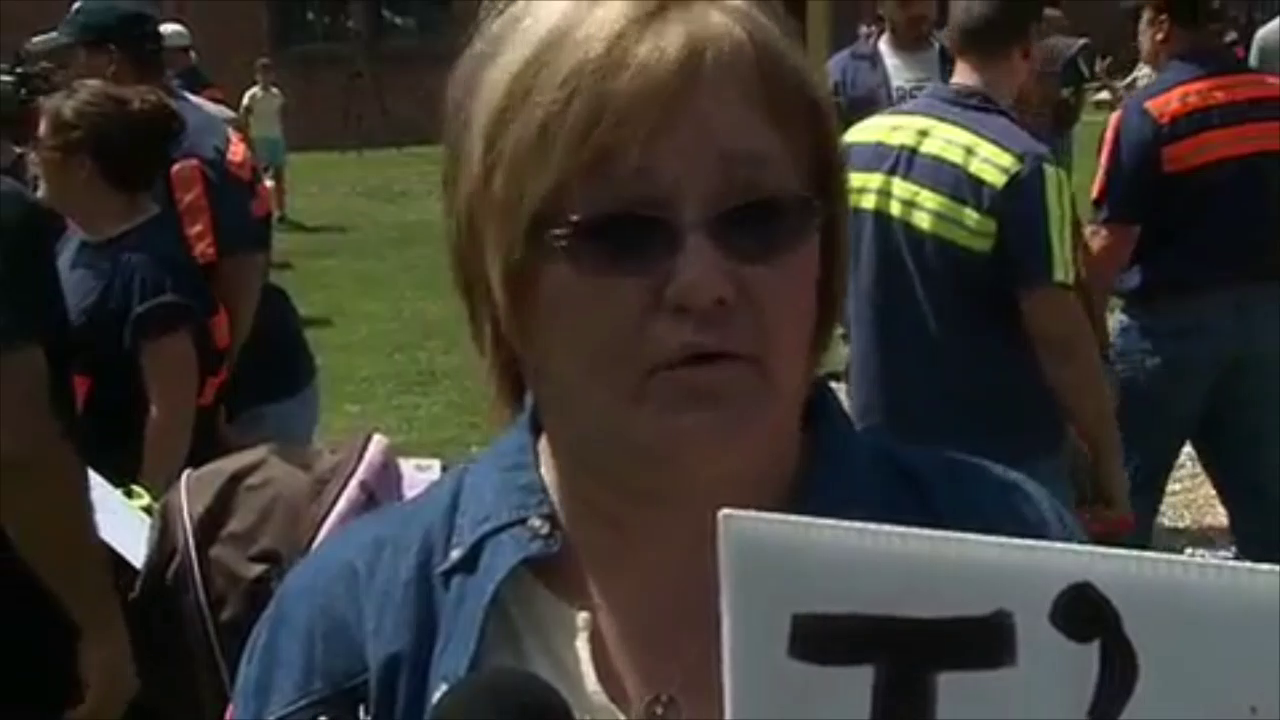
\includegraphics[width=4.2cm]{Figures/mmEcon4/frame901.png}  
\end{tabular}
\caption{Socio-Economic level - Example 4}
\begin{footnotesize}
Source: \url{https://www.youtube.com/embed/vBhvFWRLiOs?start=58&end=75}
\end{footnotesize}
\label{fig:figure1}
\end{figure}

Like in the previous example, the facial expression is one of worry and concern. Coinciding with ``this is the best paying job there is,'' is a shoulder shrug, which can be interpreted as an expression indicating innocence and helplessness, as if to say ``I can't do anything about it'' \citep{Collett2003}. In the final part of the segment, after the question (``what happens if mountaintop removal goes away?''), the facial expression turns to one of surprise with the eyebrows raised, followed by an increased pitch when answering ``we go hungry.'' 

\subsection{Cognitive Level}

The purpose of observing nonverbal communication is to better understand the meaning the speaker is trying to express. Words alone give a partial picture of that meaning, but nonverbals can provide greater insight into thoughts, feelings, and emotions. Whereas, the examples presented are primarily descriptive, this cognitive-level of analysis aims to provide some insights from cognitive science in order to interpret and tie together the various observations.

\textbf{Nonverbal Communication and the Unconscious}

The notion that nonverbals are essential to meaning and communication, is based on premises about the largely unconscious dimension of human cognition. In general terms, these premises are as follows: 

\begin{itemize}
\item Human cognition is mostly (98\%) unconscious, and is inseparable from emotion. Moreover, cognition is embodied, meaning ideas, language, and even thought are mediated by the body \citep{Lakoff2010a}. 
\item Human needs, emotions, and intentions are processed by the limbic brain. Nonverbal communication and, in particular, body language is to a large extent the expression of unconscious limbic processsing \citep{Navarro2008,T.Lamendella1977}. Gestures are expressions of embodied cognition \citep{Kinsbourne2006}.
\item In contrast to nonverbal communication, human (verbal) language abilities are more consciously driven and concentrated in the frontal lobe of the brain, which is responsible for thinking, planning, and judgment.     
\end{itemize}

In essence, cognition is mostly unconscious, it is inseparable from the body, and is expressed through embodied communication. It follows that nonverbals convey thoughts, feelings, and emotions in ways that speech alone does not. Nonverbals are often not inhibited and regulated in the same way as speech is, in the cortical and frontal lobe areas of the brain. Of course, this is a simplification. A more comprehensive review of the cognitive neuroscience of human communication is beyond the current scope. In reality, complex interactions occur between areas of the brain \citep[32]{Wood2005}. Nonetheless, the basic point is that the importance of nonverbals to discerning overall meaning is rooted in human cognition itself. Nonverbal communication is required to understand the full communicative intent, which encompasses emotions and reactions as well as thinking and judgment. 
 
While nonverbals can be deliberate and intentional, they often occur without our conscious awareness and, thus, are explicable in terms of the limbic system. Involuntary facial expressions, for instance, originate in the subcortical areas of the brain \citep[36]{Matsumoto2013}. There is also evidence to suggest that head movements encode emotional intent \citep{Livingstone2016a}. In fact, the very definition of gestures (as opposed to sign language or emblems) is that they are generated without conscious awareness \citep[9]{Beattie2016}.

\textbf{Emotional Expression}

Another key point is that nonverbal communication is closely associated with the site of emotional processing, the limbic system. As discussed in Chapter 4, sensory information is first processed by the amygdala (part of the limbic system) before further processing by the cortex. As \cite{LeDoux1994} explains:

\begin{quote}
Visual information is first processed by the thalamus, which passes rough, almost archetypal, information directly to the amygdala. This quick transmission allows the brain to start to respond to possible danger. (56)
\end{quote}

In this way, emotions serve an important cognitive evolutionary function by allowing for rapid information processing with minimal deliberation \citep{Tooby2008}. In contrast to the classical Enlightenment ideal of rational human thinking, emotions are inseparable from cognition \citep{Lakoff2010a}.

It should be noted that there is not universal agreement that nonverbal communication is a reflection of internal emotions. With respect to facial expressions, \cite{Crivelli2018} explain that, according to the behavioral ecology view of facial displays (BECV), facial displays are tools for social influence. The BECV contrasts with the basic emotions theory (BET), which holds that facial expressions reflect internal emotions. However, as \cite{Lakin2006} points out, the behavioural ecology view offers a different explanation for what we call emotions, but is still compatible with the view that facial expressions often occur without conscious awareness (65). 

One general conclusion from the examples presented in the previous section is that, in comparison with the ecological level, emotional expression seems to be more pronounced in the cultural and socio-economic levels. This conclusion is based on qualitative interpretations of clusters of nonverbals. However, to break down how one could arrive at this conclusion, we can consider facial displays in more detail.  

\textbf{Cognitive-Level Interpretation of Facial Expressions}

Psychological research has suggested there are universal facial expressions (UEs), which correspond to the ``six basic emotions'' proposed by \cite{Ekman1971} and \cite{Ekman1972}: happiness, surprise, disgust, sadness, anger, and fear. This early research also notices cross-cultural variability in facial expressions, attributed to ``display rules'' regarding emotional expression which are learned in the context of one's culture. Recent research has challenged the universality hypothesis by finding there are distinct differences in the way people from Western and Eastern cultures display and recognize the six basic emotions. There is also evidence of cultural variability in parts of the face used to express emotion. For instance, \cite{Jack2012} find that East Asian models of emotions find more intensity in the eyes. This conclusion makes sense in terms of a hypothesis that East Asian cultures learn to be more inhibited in the expression of emotion and the eyes, which are generally subject to less voluntary control than the mouth \citep{Mai2011}, are better indicators of emotional expression.

In the context of the examples presented, the primary implication is that interpretation of facial expressions is just that: an interpretation. There are some general, perhaps universal characteristics, but the expression and interpretation of emotion also varies with the culture of speakers/observers. One way to account for cultural variability, however, is to pay particular attention to the eyes.

In the ecological-level examples some facial expressions were noted. However, these can generally be interpreted as expressing lower degrees of emotion than those seen at the other levels. In the first example, for instance, the speaker has what might be described as a ``neutral face,'' characterized by either a low degree of emotion or an expression in its own right whose emotional meaning is contextual \citep{Carrera-Levillain1994}. Given the context of the first example (scientist discussing research), the neutral expression fits with the social and professional expectations of the communicative context. Accordingly, we might conclude that there is relatively low emotional reaction in this segment. This conclusion is supported by the content of the speech, which indicates the speaker is also engaged in non-binary thinking by outlining that there are grey areas about the ecological impacts of deep sea mining. Non-binary thinking is an indication that, rather than an automatic response from the amygdala, there is emotional modulation via the cortex, which manifests as exploring and considering different options or reactions \citep{Wood2005}.    

Another indication of emotional modulation is the upward motion of the eyes, which can be seen in the ecological as well as the cultural examples. This, again, is a possible indication of engagement with rational thinking and the cortex (as opposed to the automatic response of the amygdala). Research suggests looking upward is associated with spatial and verbal memory recall \citep{Nespoulous2014}. Whereas emotional ``fight or flight'' responses dilate the pupils to increase visual information, the opposite might also be the case when engaging in abstract thinking with the prefrontal cortex; that is, a relaxing of the gaze and limiting the visual information in order to free up cognitive processing for information retrieval.

In the cultural-level examples, we also see evidence of more emotional responses. The higher degree of emotion is not surprising given that these speakers are addressing identity and intergroup relations amid sensitive topics. As mentioned, cultural Example 2 contains a ``sneer,'' which is often said to be an expression of contempt \citep{Izard1988}. In cultural Example 3, the speaker displays a high blink frequency and blink duration, which is a possible sign of negative emotional states including stress \citep{Haak2019} and fear \citep{Maffei2019}. Thus, at the cultural level we see a mix of emotions by way of facial expressions.

Emotional facial expressions are perhaps most pronounced at the socio-economic level. Unique to this level are the expressions of sadness, worry, and concern. Sadness is generally associated with oblique eyebrows and pulling down of the lip corners \citep{Duran2017}. This expression is apparent in socio-economic Example 2, which is unsurprising given that the topic in this segment is unemployment and economic hardship. Also, in the same segment we see watery eyes and possible tearing. In adults who generally have developed empathy, tearing is often triggered by the suffering of others \citep{Murube1999}. In the same example, we see listeners exhibiting similar emotional responses. At the cognitive-level, the listener responses can be seen as an example of how emotions elicit a ``mosaic'' of mirror neurons causing the observer to experience similar feelings as the person who expressed the emotion \citep{Bastiaansen2009}. 

\textbf{Cognitive-Level Interpretation of Gestures}

In addition to different facial expressions, the three levels of analysis (ecological, cultural, and socio-economic) also exhibit differences in the gestures displayed. As mentioned, in the ecological-level there is a notable use of iconic gestures, which closely reflect literal spoken words, at the interface of imagistic and linguistic representation \citep{Ozyurek2010}. As speakers begin to address cultural and socio-economic topic, the gestures become less iconic and more metaphorical. At these levels, the emotional intensity increases. How we can interpret something that is seemingly subjective (i.e. the emotional intensity of gestures) is outlined by \citeauthor{Kinsbourne2006} (\citeyear{Kinsbourne2006}) as follows: 

\begin{quote}
When gestures are driven by emotion they become less discrete, and may
occur in concert with postural shifts and facial expressions that incidentally emphasize and clarify the meaning that is being communicated. (208)
\end{quote}

In other words, when a speaker is more emotional, their gestures often increase in amplitude, pace, or frequency. That said, it is not gestures alone that convey the emotion, but gestures in conjunction with other nonverbal signals. 

The ``discrete'' gestures we see in the ecological examples communicate spatial relationships in close relation to semantic information. The speakers are often describing physical processes, such as the directional pointing in Example 2 or water well spigot inspection (Example 3). These gestures are controlled, deliberate, and match the literal semantic information. 

By contrast, in the cultural examples gestures become more metaphoric. They emerge in conjunction with more abstract topics including culture, fighting back, or in-group/out-group identities. The same can be said with respect to the socio-economic examples, but with an important distinction: the cultural examples are often expressions of power, confidence, and assertion. For instance, we see palm down motions, pointing, a fist pump, and thumb displays. However, in the socio-economic examples we are more likely to see expressions of hopelessness and innocence. These include several instances of the palm open ``pleading'' gesture, as well as the shoulder shrug, and the hand covering the chest.      

\textbf{Summary of the Cognitive Level}

The observed trends in facial expressions and gestures suggest that different cognitive responses are exhibited at different levels of discourse. The ecological level exhibits more verbal and spatial reasoning and does not appear to trigger emotional responses. In other words, the ``fight or flight'' emotional responses of limbic system and subcortical areas of the brain are being mediated. The cultural level seems to trigger emotions, but these are generally high confidence, one could even argue dominant, nonverbal signs. This might be attributed to in-group identities that are being asserted. Finally, the socio-economic level is more likely to display low confidence gestures. The sense of exclusion and vulnerability in the face of threatened livelihoods is one possible explanation for these responses.

\section{Summary \& Conclusions}

Nonverbals are not merely an important part of communication to consider alongside speech; they are inseparable from the message itself. This chapter aimed to look at communication in a holistic sense, with verbal and nonverbal communication as part of an integrated flow. However, if there is a point at which we can distinguish nonverbals from verbal communication, it is with respect to their relation to cognition and emotions. As \citeauthor{Beattie2016} (\citeyear{Beattie2016}) points out, with nonverbal communication ``meaning has not been controlled and self edited by the speaker'' (16). In other words, the nonverbal messages are reflective of mental processes and emotions, in ways that words alone are not.

The most notable conclusion from this chapter is that different discursive levels corresponded to different types of nonverbal displays, as outlined in Table 5.2 below. These differences can be summarized as follows:

\begin{itemize}
\item Speakers at the ecological level generally show less facial expression. Gestures are predominantly iconic and depicted physical/spatial processes. Compared to the other levels of analysis, intonation and stress are less pronounced.  

\item Speakers at the cultural level display more power and confidence gestures, including pointing (to add emphasis), thumb displays, and fist pumping. Gestures are more metaphoric than in the ecological level, depicting abstract concepts such as God, culture, identity, and fighting back. Contempt and agitation are displayed, at one point by the contempt expression (raised side of mouth) as well as the backwards thumb gesture on another occasion.

\item The socio-economic level displays a high degree of emotion, often expressed in the eyes. Universal facial expressions of fear and sadness can be seen in the speakers and, in one case, among listeners. Gestures also indicate hopelessness and innocence, such as the palm open ``pleading'' gesture as well as the shoulder shrug.  \end{itemize}

\begin{table}[H]
\centering
\begin{footnotesize}

\begin{tabular}{ | P{3cm} | P{3cm}| P{3cm} | P{3cm}| }  
\hline
\textbf{Level}          & \textbf{Gestures} & \textbf{Facial Expression} & \textbf{Paralanguage} \\ \hline
\textbf{Ecological}     &  Iconic; depicting physical processes (directional pointing, hand motions)                & Minimal emotional expression; some eyes looking upwards (thinking expression)                           & Minimal stress and intonation                      \\ \hline
\textbf{Cultural}       & Metaphoric; depicting power, confidence, and assertion (palm down, pointing, fist pump, thumb displays)                 &    Contempt displays; anger; agitation (sneer, higher blink rate, audible inhalation/exhalation)                         &  Stress on key points; more variation in speed of speech                     \\ \hline
\textbf{Socio-Economic} &  Hopelessness and innocence (palm open, shoulder shrug; hand on chest)                &     Sadness, concern, worry, fear (raised eyebrows, teary eyes, eyebrows pulled together)                        & Stress; intonation; more changes in pitch                       \\ \hline
\end{tabular}
\caption{Summary of nonverbal communication observations}
\label{tab:my-table}
\end{footnotesize}
\end{table}

It appears that emotions and unconscious attitudes vary when it comes to environmental issues. Specifically, when one's cultural identity or socio-economic status are at stake, these attitudes intensify. When ecological issues are decontextualized from identities or livelihoods, the opposite seems to occur. \citeauthor{Beattie2016} (\citeyear{Beattie2016}) discusses similar observations in terms of implicit and explicit attitudes towards environmental issues:  

\begin{quote}
    The vast majority of people say that they really do care about environmental issues...yet... \textit{sometimes} there is something about the form and nature of their hand movements...which might suggest otherwise. (19, original emphasis)
\end{quote}

In other words, there is a discrepancy between what people consciously know they \textit{should} care about, and how they unconsciously feel. 

This discrepancy has great relevance when it comes to raising awareness about, and addressing, ecological issues. The implication is that communication matters a great deal when it comes to the environment. Specifically, mobilizing people to address ecological issues will depend on framing these issues in a way that speaks to their implicit, unconscious attitudes. From a cognitive science perspective, \citeauthor{Lakoff2010a} (\citeyear{Lakoff2010a}) makes this point and advances some implications for environmental communication, namely

\begin{itemize}
\item The importance of discussing environmental issues in terms of moral values.
\item The efficacy of stories and narratives as opposed to statistics and bland facts.
\item The necessity to address everyday concerns and avoid technical jargon. (79-80) 
\end{itemize}

The observations in this chapter support these points. However, the point about ``moral values'' might be expanded to encompass cultural identity and worldviews. The examples in this chapter show multiple ways in which culture emerges in environmental debates, and how issues becomes impassioned when this occurs. Also, the necessity to address ``everyday issues'' is underscored by the importance of framing issues in terms of economic livelihoods.     
